\documentclass[a4paper,doc,draftfirst]{apa6}
\usepackage[utf8]{inputenc}
\usepackage[UKenglish]{babel}
\usepackage{pdfpages}
\usepackage[style=apa,sortcites,sorting=nyt]{biblatex}
\DeclareLanguageMapping{UKenglish}{ukenglish-apa}
\graphicspath{{./}}
\usepackage[toc,page]{appendix}

\title{CS3099 Major Software Team Project}
\shorttitle{JH project report}
\author{Keanan Frazer, Bethany Gillam, Liam McMenemie, Christa-Awa Köllen, Jack Neilan}
\leftheader{Frazer, Gillam, McMenemie, Köllen, Neilan}
\affiliation{University of St Andrews}
\authornote{Authors were members of project group G.}
\note{Submitted 2017-04-18}

\abstract{\textbf{The abstract should be about 100 words long.}
Settlers of Catan is a popular strategy board game, involving extensive communication, collaboration, and strategy. To design a successful implementation of the game would involve a clear, well-defined protocol for communication between a game client and hosting server, that could capture these core elements of the game while maintaining and conveying a similar experience. The entire year group was split into groups of 4 or 5, and were tasked with implementing Settlers of Catan, functioning AIs which could play the game, and basing the entirety of the implementation off of a common group protocol which was up to the groups to coordinate and develop.
}
\begin{document}
\maketitle




\section{Declaration}
We declare that the material submitted for assessment is our own work except where credit is explicitly given to others by citation or acknowledgement. This work was performed during the current academic year except where otherwise stated. The main text of this project report is \textbf{NN,NNN} words long, including project specification and plan.

In submitting this project report to the University of St Andrews, we give permission for it to be made available for use in accordance with the regulations of the University Library. We also give permission for the report to be made available on the Web, for this work to be used in research within the University of St Andrews, and for any software to be released on an open source basis.

We retain the copyright in this work, and ownership of any resulting intellectual property.




\newpage
\tableofcontents
\newpage




\section{Introduction}
\textbf{Describing the problem the team set out to solve and the extent of its success in solving it. The section should outline key aspects of the project for the reader to look for in the rest of the report.}

This practical was meant to challenge one’s ability to effectively work in a group, and to structure a large scale software project to meet a series of vaguely-defined end goals. To accomplish this, the groups needed to effectively organise tasks amongst themselves, interface with other teams to develop a standard protocol compatible with all implementations, set and adhere to self-imposed deadlines, and finally to deliver a product by the final date. The task was to build Settlers of Catan, a strategy board game, and have it equipped with AIs, the ability to play games over the network, the ability to network with other teams and to of course have a working implementation of Catan’s basic rules and game logic. All of this was to be accomplished at the discretion of the group, through experimentation and refinement where necessary, as well as through the successful delineation of tasks amongst the group’s constituents.

\paragraph{Beginning the project}
To begin the project, the vague requirements were broken down and elaborated on, so that we could have a more complete idea of our team's goals and how we intended to achieve them. We also set several extension features which we would have liked to accomplish, such as implementing expansion packs or the larger board which could accomodate 5-6 players. This involved specifying the ways in which we wanted our program to operate, so that architecting the actual implementation involved less subjectivity. We began by setting out to structure the project in as modular of a manner as possible, so as to be able to re-use as much code as we possibly could. This involved more planning in the beginning, but made our lives much easier when figuring out how the different components were to interact (AIs, networking, etc.). We initially knew the best way of going about structuring the project was if the Server didn't discriminate between the nature of its connections; that is, the server shouldn't care -- or even know -- whether its sending or receiving a message from an AI, a player, or the network. We also knew we wanted to write the project with a language or framework specifically tailored for gaming, and that is was not to be a web-app. The latter decision followed from wanting our game to be as accessible as possible, in that it could be played without any internet connection whatsoever, while still retaining the platform independence and flexibility that a web-application offers. The decision rested between C\# and Unity, Lua and the Love2D engine, or Java and libGDX, which is what was used for 'Minecraft.' Originally, we had chosen to use Lua, however it did not have a good library for handling protocol buffers. Given that we ended up basing the entirety of the client / server interaction around protocol bufffers, we opted to switch to Java. This was chosen due to everyone's familiarity and comfortability with Java development, and libGDX's and Java's ability to be run regardless of platform. C\# was decided against as there was no easy way of getting Unity to run on the lab machines, and not everyone in the group was comfortable with switching to working with windows and .NET. 

\paragraph{What this implementation achieves}
This implementation achieves all of the basic requirements, including the ability to play with AIs (either locally or remotely), the ability to play as an AI or a player, the ability to play an off-line game (local server achieved via threading, and AIs run directly from it), the ability to play as a player networked into a remote server, and the ability to network with other groups’ implementations. The UI and front-end utilise libGDX for rendering of art and graphics, and the server is exposed through the abstraction of the actual implementation of a Client’s connection. For example, the server is able to be run with remote players through Java’s standard TCP sockets, or alternatively through a local connection all via the same code and turn flow; in the case of it being locally run from a client, the server is capable of being run on a different thread (spun off of a ‘LocalClient’ or ‘LocalAIClient’) complete with complex, concurrent data structures and semaphores to ensure the correct behaviour. Conversely, the server is capable of being run as a stand-alone program, where clients can simply connect via TCP sockets. Given that connections are abstracted over, these features can all be mixed and matched, depending which components are plugged in with the Server (e.g. a completely offline game with four AIs, an offline game with one human player and three AIs, or an online game with a human player, and any combination of remote clients and local AIs to fill in the blanks. Java is used throughout the entire project, for the coding of the game logic, the server, and the client.

\paragraph{Running the program}
\begin{figure}[hbtp]
      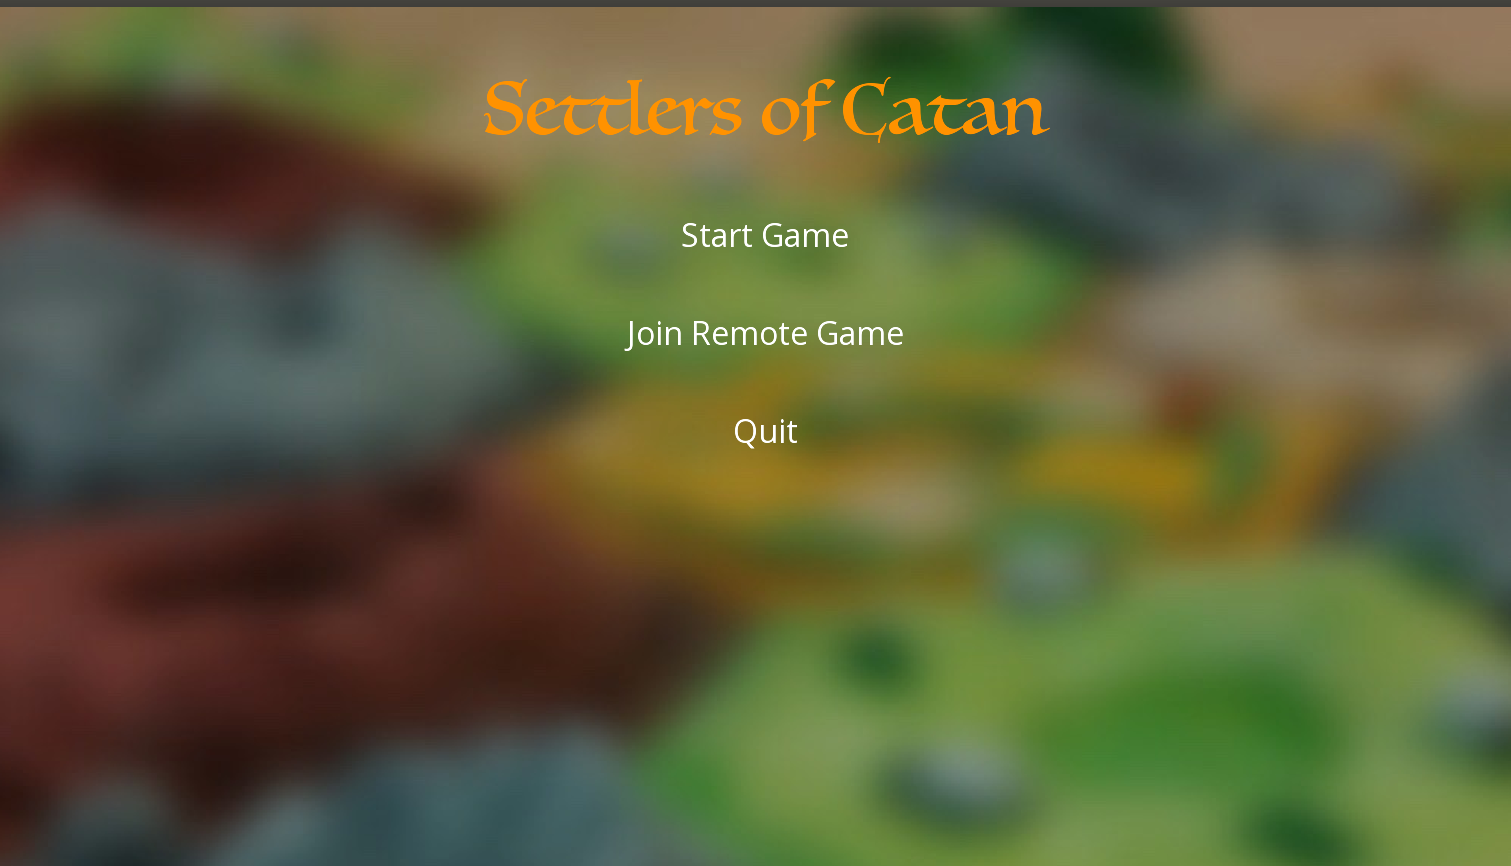
\includegraphics[width=\textwidth]{MainMenu}
      \caption{Main Menu for running the program}
\end{figure}
The project is dependent on Google Protocol Buffers v3.2, Java8, and libGDX v1.9.5. The entire project utilises gradle to simplify running the program from a fresh clone of the repository; instead of the user having to bother with ensuring they have the aforementioned libraries installed, simply running './gradlew run' from the command line within the main directory will build the project, download all dependencies, compile the protocol buffer files into Java files, and then spin up the user interface to begin program execution. From within the program, the user can choose to join a remote game, or start a local game in which they can choose the number of AIs and their respective difficulties. In this way, the user needn't worry about running multiple programs just to get a game to start; all they need to do is enter in their desired settings, and the game will spin up the relevant threads to run the different code (AIs, Server, Client, GUI, etc.).




\section{Project details}
\textbf{Summarising the achievements of the project, and discussing those aspects of the project that are of particular interest: the main ideas of the design, unusual design features, special algorithms and data structures, odd implementation decisions, novel user interface features, etc.}

\subsection{Protocol design}
\begin{figure}[hbtp]
      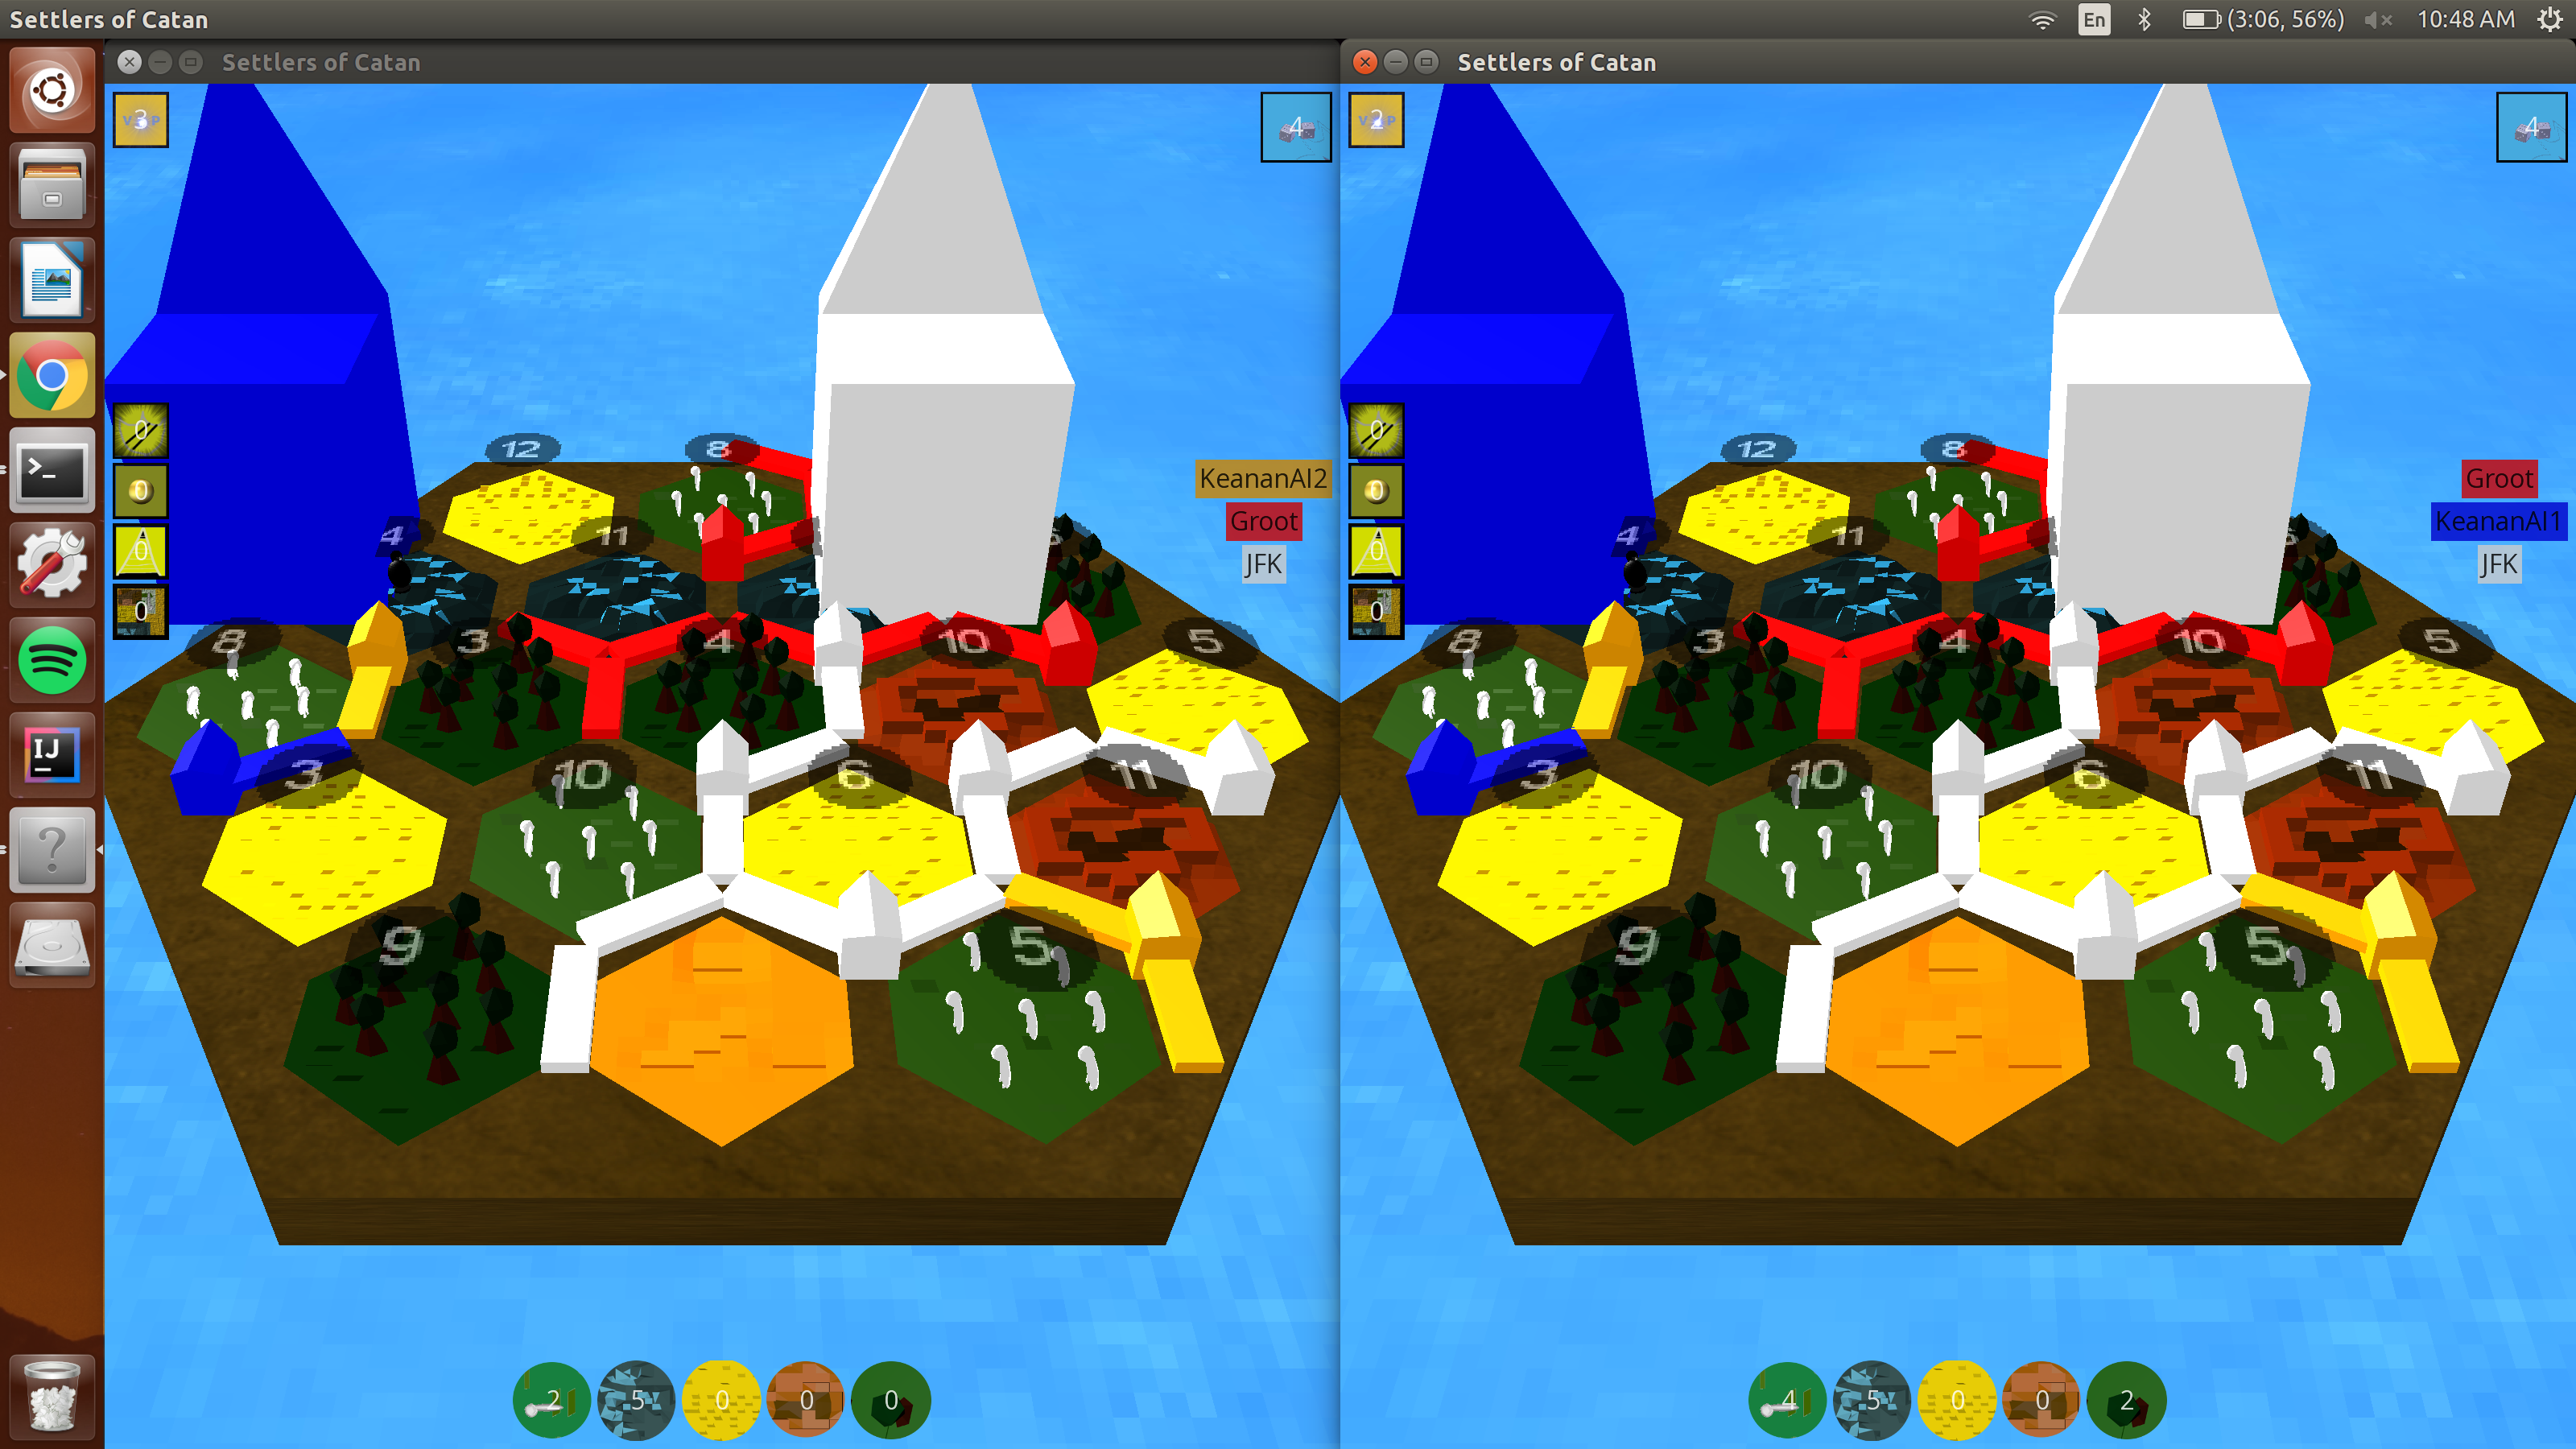
\includegraphics[width=\textwidth]{finishedAIGame}
      \caption{Networking game between two of our AIs and two of Group I's}
\end{figure}
Early on, it was decided that the intergroup protocol would be implemented via Google’s Protocol Buffers, as opposed to JSON. This is due to the inherent advantages protocol buffers entail, including much more compressed message size, and an extra level of validation and definition in what the protocol messages entailed and had to be. This is in contrast to JSON, where ultimately someone could put a string in the place of an integer, meaning there is a substantially higher chance for error, and therefore a need for a large amount of message validation and sanity-testing.

The protocol structure is as follows: the overarching message type is a ‘Message.’ A ‘Message’ has a ‘one-of’ field, which simply means that a message can be either a ‘Request’ or an ‘Event.’ When compiled, 'one-of' fields involve an implicit enum which tells the receiving program which field is set. When switched upon, a user can easily identify the type of message, and discern how to process it. These message types represent communication from the client to the server, and the server to the client, respectively. An event can be sent either just to the sender, in the case of secret information or an error occurring in the previous request, for example, or can be sent to every player as a receipt of a valid move that was carried out. An example of secret information would be the exact contents of a card which was stolen, or which development card ended up being bought. In these cases, the original event is sent to the player in question (if a steal, this could be sent to both players), and then the relevant information is obscured before being sent to other players. For example, in the case of stealing a resource, the resource type is merely altered to be ‘Resource.Kind.Generic’.

A ‘Request’ has a one-of field for each defined request type (including building a settlement, road, or city, playing a development card, buying a development card, starting a trade, choosing a player to steal from, choosing a resource, etc). An ‘Event’ is similar in that it has a ‘one-of’ field, meaning it can take the form of any number of ‘Event’ types which roughly correspond to the ‘Request’ types (including settlement built, city built, road built, resource stolen, development card bought, development card played, trade occurred, etc.). An ‘Event’ also has an ‘instigator’ field which simply entails the ‘ID’ of the player who sent it. While this is almost always the current player, including this information was important for debugging purposes and move validation.


\begin{figure}[hbtp]
      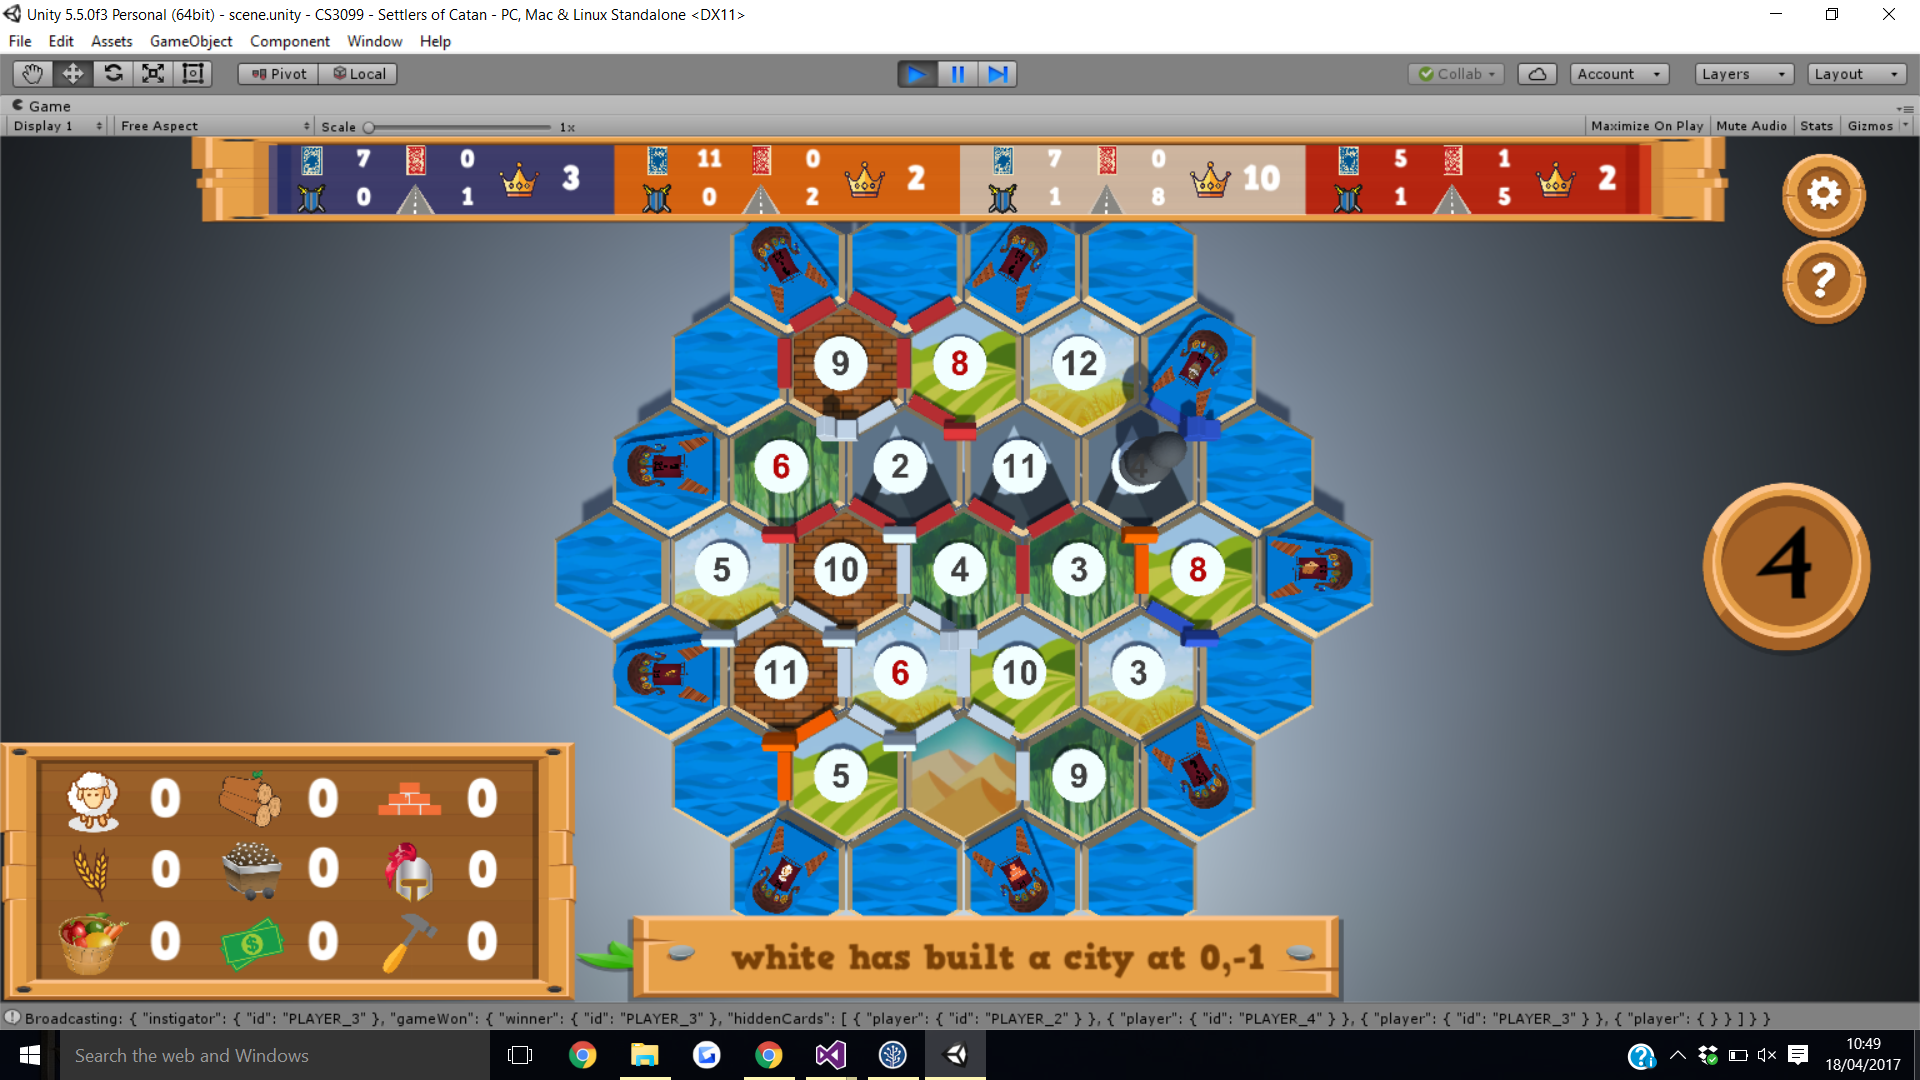
\includegraphics[width=\textwidth]{GroupI}
      \caption{Same view of the above game from Group I's perspective}
\end{figure}

This implementation is coded fundamentally in terms of this group protocol, as it involved the simplest approach, and less boilerplate code for validation and message translation. The overall philosophy behind the group protocol involved keeping the information sent to be as minimal as possible, and to best reflect the actual turn flow of a Settlers of Catan game in real life. This involved single "moves" entailing several separate message types which need to be sent in sequence. This was chosen as it best represents the flow of a game; when a user decides to play a knight development card, they then tend to deliberate for a bit before choosing where to place the robber, and consequently who to steal from. All different moves are broken down into their logical components, simplifying the protocol and allowing for message re-use between different types of turns. For example, in playing a 'Year of Plenty' card, the user then needs to choose two resources. The 'CHOOSERESOURCE' message is used in this instance, as well as when choosing a resource when playing a 'Monopoly' card. The primary consequence of structuring the protocol in this manner meant that the client would be 'fat,' in that it would need to replicate a lot of the logic on the server, as the server only sends the bare minimum relevant information.

\section{Board design}
\begin{figure}[hbtp]
      \includegraphics[width=\textwidth]{BoardDesign}
      \caption{Class diagram showing the different components of a HexGrid}
\end{figure}
The board is the root of what “Settler of Catan” is, and as such, needed to be as efficient as possible so the rest of the implementation did not suffer. The coding and representing the board was worked on first. The HexGrid entails a Hash map of ‘Point’ objects to ‘Hex’ objects, a hash map of ‘Point’ objects to ‘Node’ objects, a list of ‘Edge’ objects, and a list of ‘Port’ objects, a specialisation of ‘Edge.’ It also maintains which hex has the robber. To construct the hash maps and data structures in this manner is expensive in terms of time, but results in exceptionally fast retrieval. This was deemed to be a fair trade-off, as retrieval of objects will occur infinitely many more times than the initial set-up. Due to this, it would present itself as a notable inefficiency in the data structure to have lists as opposed to hash maps. Likewise, the board is generated long before anyone even requests it anyway, making the slightly longer set-up time negligible.

The ‘Point’ class was used as the key type for the aforementioned hash maps due to one particular quality: the Point class is hashed purely based on its ‘x’ and ‘y’ integer fields. In this way, hashCode(new Point(1,1)) == hashCode(new Point(1,1)). This quality makes ‘Point’ act a bit like a tuple in this instance, which made it an excellent choice to represent the coordinates of the board, and to be keys for the data structures maintaining it; for example when coordinates are received over the network as a part of a certain move, say a ‘BUILDCITY’ move, then the node can easily be retrieved through extracting the x and y values, and doing: grid.getNode(x, y). Then further checks can be performed and the move can be validated and carried out. Another important note of the design of the board involves the abstraction over elements that go into a HexGrid. To start with, a ‘BoardElement’ is used to describe anything on a board, which includes an ‘Edge’ or a ‘GridElement.’ A ‘GridElement’ is used to define anything on the grid that can be defined with x and y coordinates (‘Hex’ and ‘Node’). These abstractions are leveraged in forming a list of potential, valid objects that can be built upon (reference MoveProcessor.java), for example, and in storage of objects in a single data structure (since they all implement BoardElement). This is utilised when generating valid moves based on the game state, which is used in the UI as well as in the AI’s move decision process.

\subsection{Instantiating a new Board}
\begin{figure}[hbtp]
      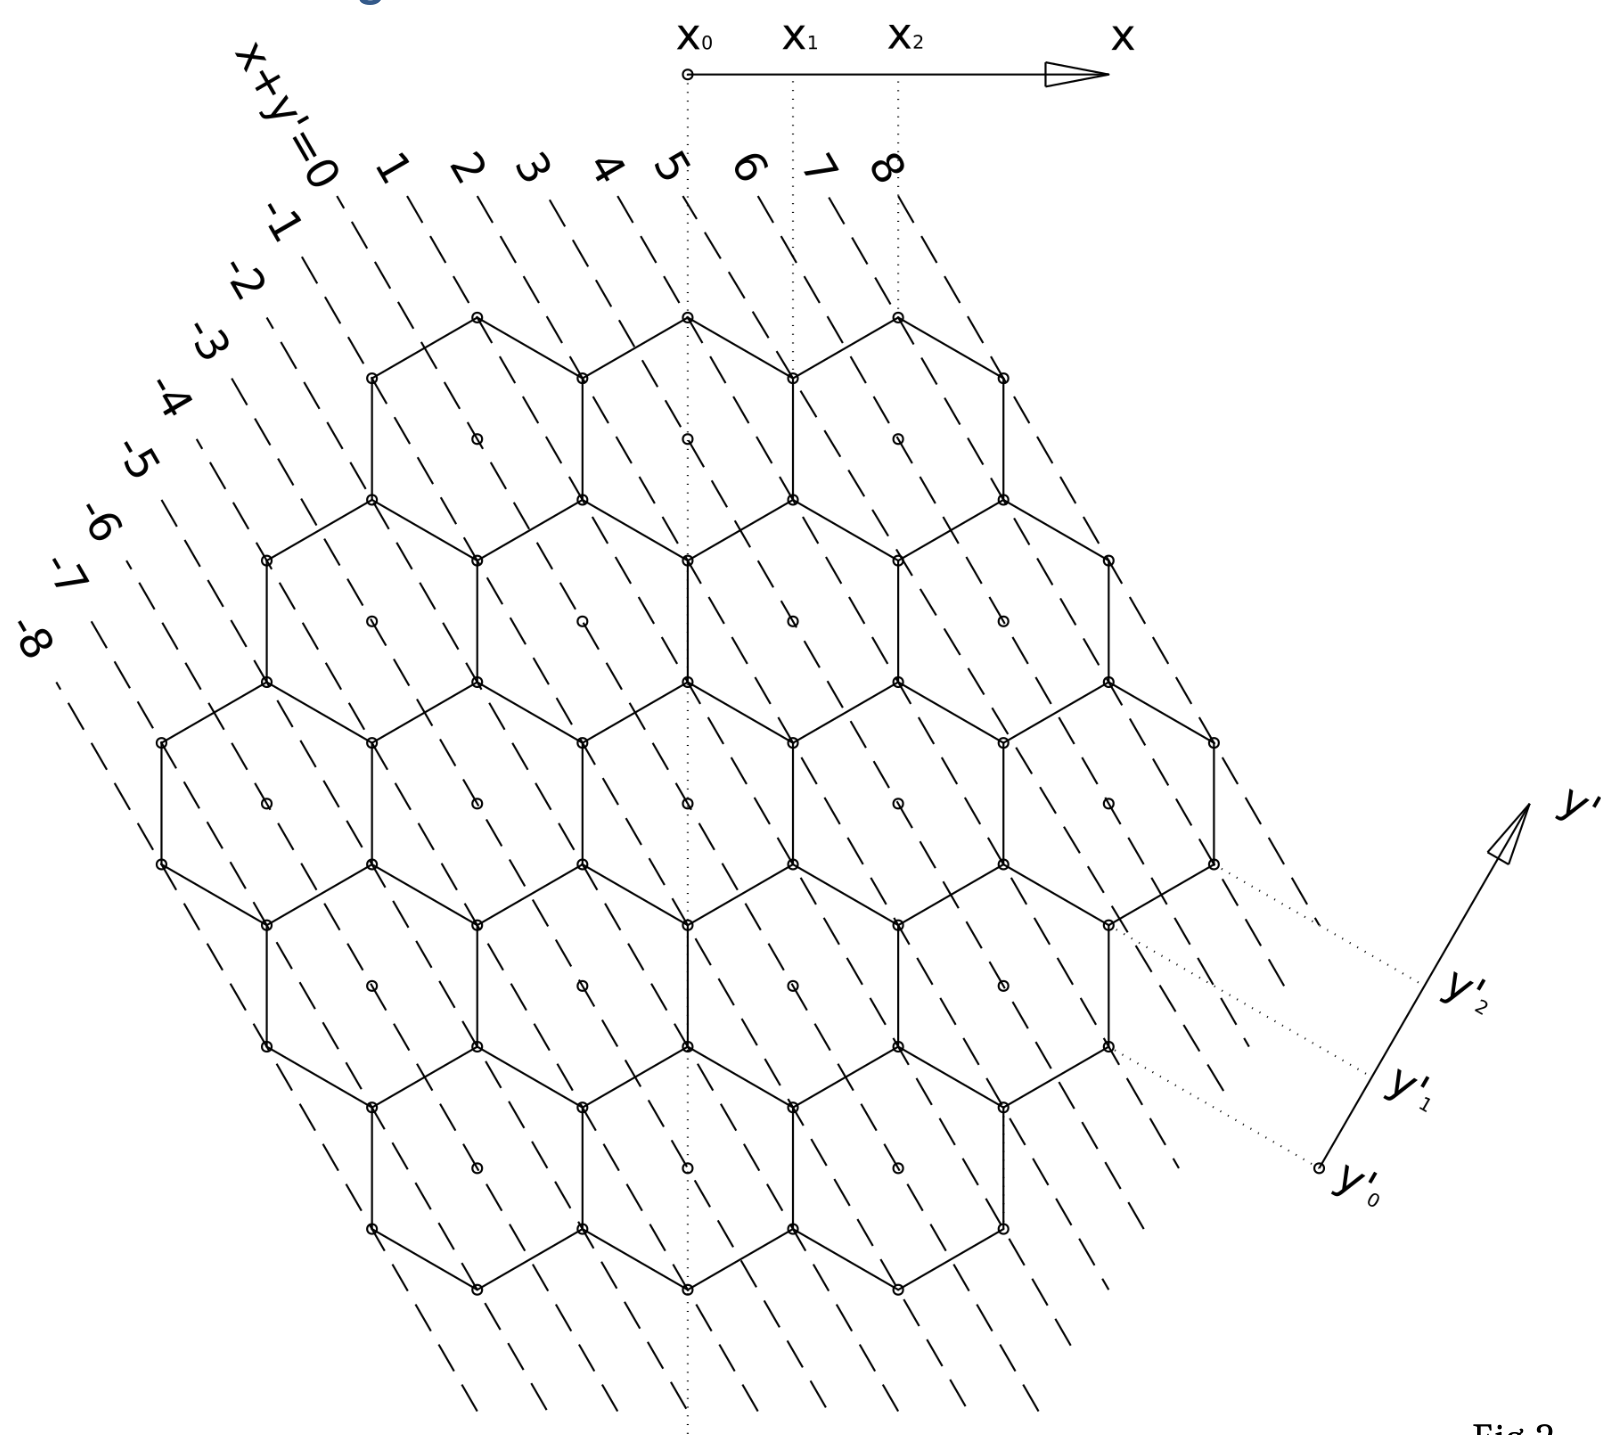
\includegraphics[width=\textwidth]{board}
      \caption{Catan coordinate system}
\end{figure}
Despite the data structures for the board making sense, populating them with values became a lot trickier. The coordinate system used in the group protocol ended up being the most appropriate for our implementation, as it defines Nodes and Hexes on one coordinate system, allowing for less coordinate translation and object manipulation all around. This is due to the way in which the x and y axes are defined relative to the hex grid; as such, the board, its boundaries and which coordinates represent a ‘Node’ vs a ‘Hex’ are all formalised mathematically. In this way, one can set up nodes and hexes through two nested for loops, systematically iterating from one end of the coordinate system to the other. Using a simple check (x \% 3 == 0 indicates a ‘Hex’), the various nodes and hexes can be created easily. If the coordinate represented a ‘Hex’, then a chit and a resource are randomly assigned based upon a statically-created map of remaining resources and chits. From there however, linking up the nodes and hexes in their complex web of relationships was a lot trickier. For this, all neighbours of a ‘GridElement’ are retrieved. A ‘neighbour’ of a ‘GridElement’ entails all other ‘GridElement’ objects which have a distance between $1$ and $-1$ in their x coordinates, and the same with their y coordinates (with the exception of both differences being equal). This results in all 6 neighbours: for a hex, it retrieves 6 nodes, and for a node it retrieves between 1 and 3 hexes and 2 or 3 nodes (depending upon board location). In having the list, then mutual references can be established, allowing for simpler algorithms down the road (e.g. retrieving the resource type from a hex adjacent to a settlement (node), useful for resource allocation); the neighbours are simply iterated through, forming all appropriate relationships between objects on the board. If the neighbour is a node, then an edge is created (if not already created previously) as well. With nodes and hexes having their references established and ‘Edge’ objects having been created, ‘Port’ objects needed to then be created. Ports can be ascertained by the mathematical boundaries of the board, and the port types are randomly distributed amongst the various fixed positions. 

\section{Game design}
A ‘Game’ is a raw game-state class used to define the information common to the representation of state on both the client and server sides. The idea of a game is modelled using inheritance; Game is the core representation of a game (including a board, basic information about players, fundamental methods, etc.), while ‘ServerGame’ is a specialisation which includes other server-specific information and methods that go into running the game (i.e. resource allocation, changing turns, joining games, etc.), and ‘ClientGame’ is a specialisation which includes client-specific information and methods. ‘Game’ and all of its specialisations simply add the capabilities to manipulate the underlying board (a ‘HexGrid’ object), and information held in instances of ‘Player.’ In this way, they add the notion of “state” on top of the core representation of “Settlers of Catan.” This approach allowed for the most amount of code re-use possible, since the client and server need to have the same underlying notion of a game state anyway. In this way, ‘Game’ also entails a lot of common functionality that both the server and client need, including methods to check if a road was broken, to update largest army, or add a new player, for example. The ‘Game’ also entails a grid and basic structures for maintaining players, the bank, ids, etc.

\subsection{Differences between the Client's and Server's view of a Game}
The primary difference between these two specialisations of ‘Game’ is the way in which they interact with the larger game flow; that is, ‘ServerGame’ is essentially ‘Game’ with additional logic to process requests, with ‘ClientGame’ being similar except with logic for processing events. Likewise, a ‘ServerGame’ acts as the authoritative view for the entire instance of “Settlers of Catan,” across all players, while ‘ClientGame’ acts a ‘view’ on this overall state through the perspective of a Client. ‘ServerGame’ essentially entails a series of functions which correspond to each ‘request’ type defined in the intergroup protocol. These methods all entail extensive exception usage which, when thrown, indicate to the server’s MessageProcessor (which called this method) that the request failed. If so, then the exception is caught, and an error event is subsequently set up and sent back to the corresponding client. This exception handling allows for rules to be iterated upon / altered in a very easy, transparent way. Likewise, it provides a uniform, understandable way of indicating when something goes wrong. With all errors going down the same code path, regardless of origin, there is far less code re-use and less boiler plate code for checking if methods return ‘null’ instead of a proper value, etc. This system also involves incredibly detailed error messages which can be sent back to the ‘Client’  in question. Some examples of exceptions being thrown are if a user cannot afford something, if the bank cannot afford something, and if an object already exists where you are trying to build. Other, similar edge cases being covered in this way as well. This is in contrast to ‘ClientGame,’ which entails a series of functions which correspond to each ‘event’ type that is defined in the intergroup protocol. These methods process each event type and alter the given game state and / or player data, from the perception of the ‘Client’ at hand. This has similar exception handling, except to a lesser extent given that the server has to be trusted as having the authoritative view.

\begin{figure}[hbtp]
      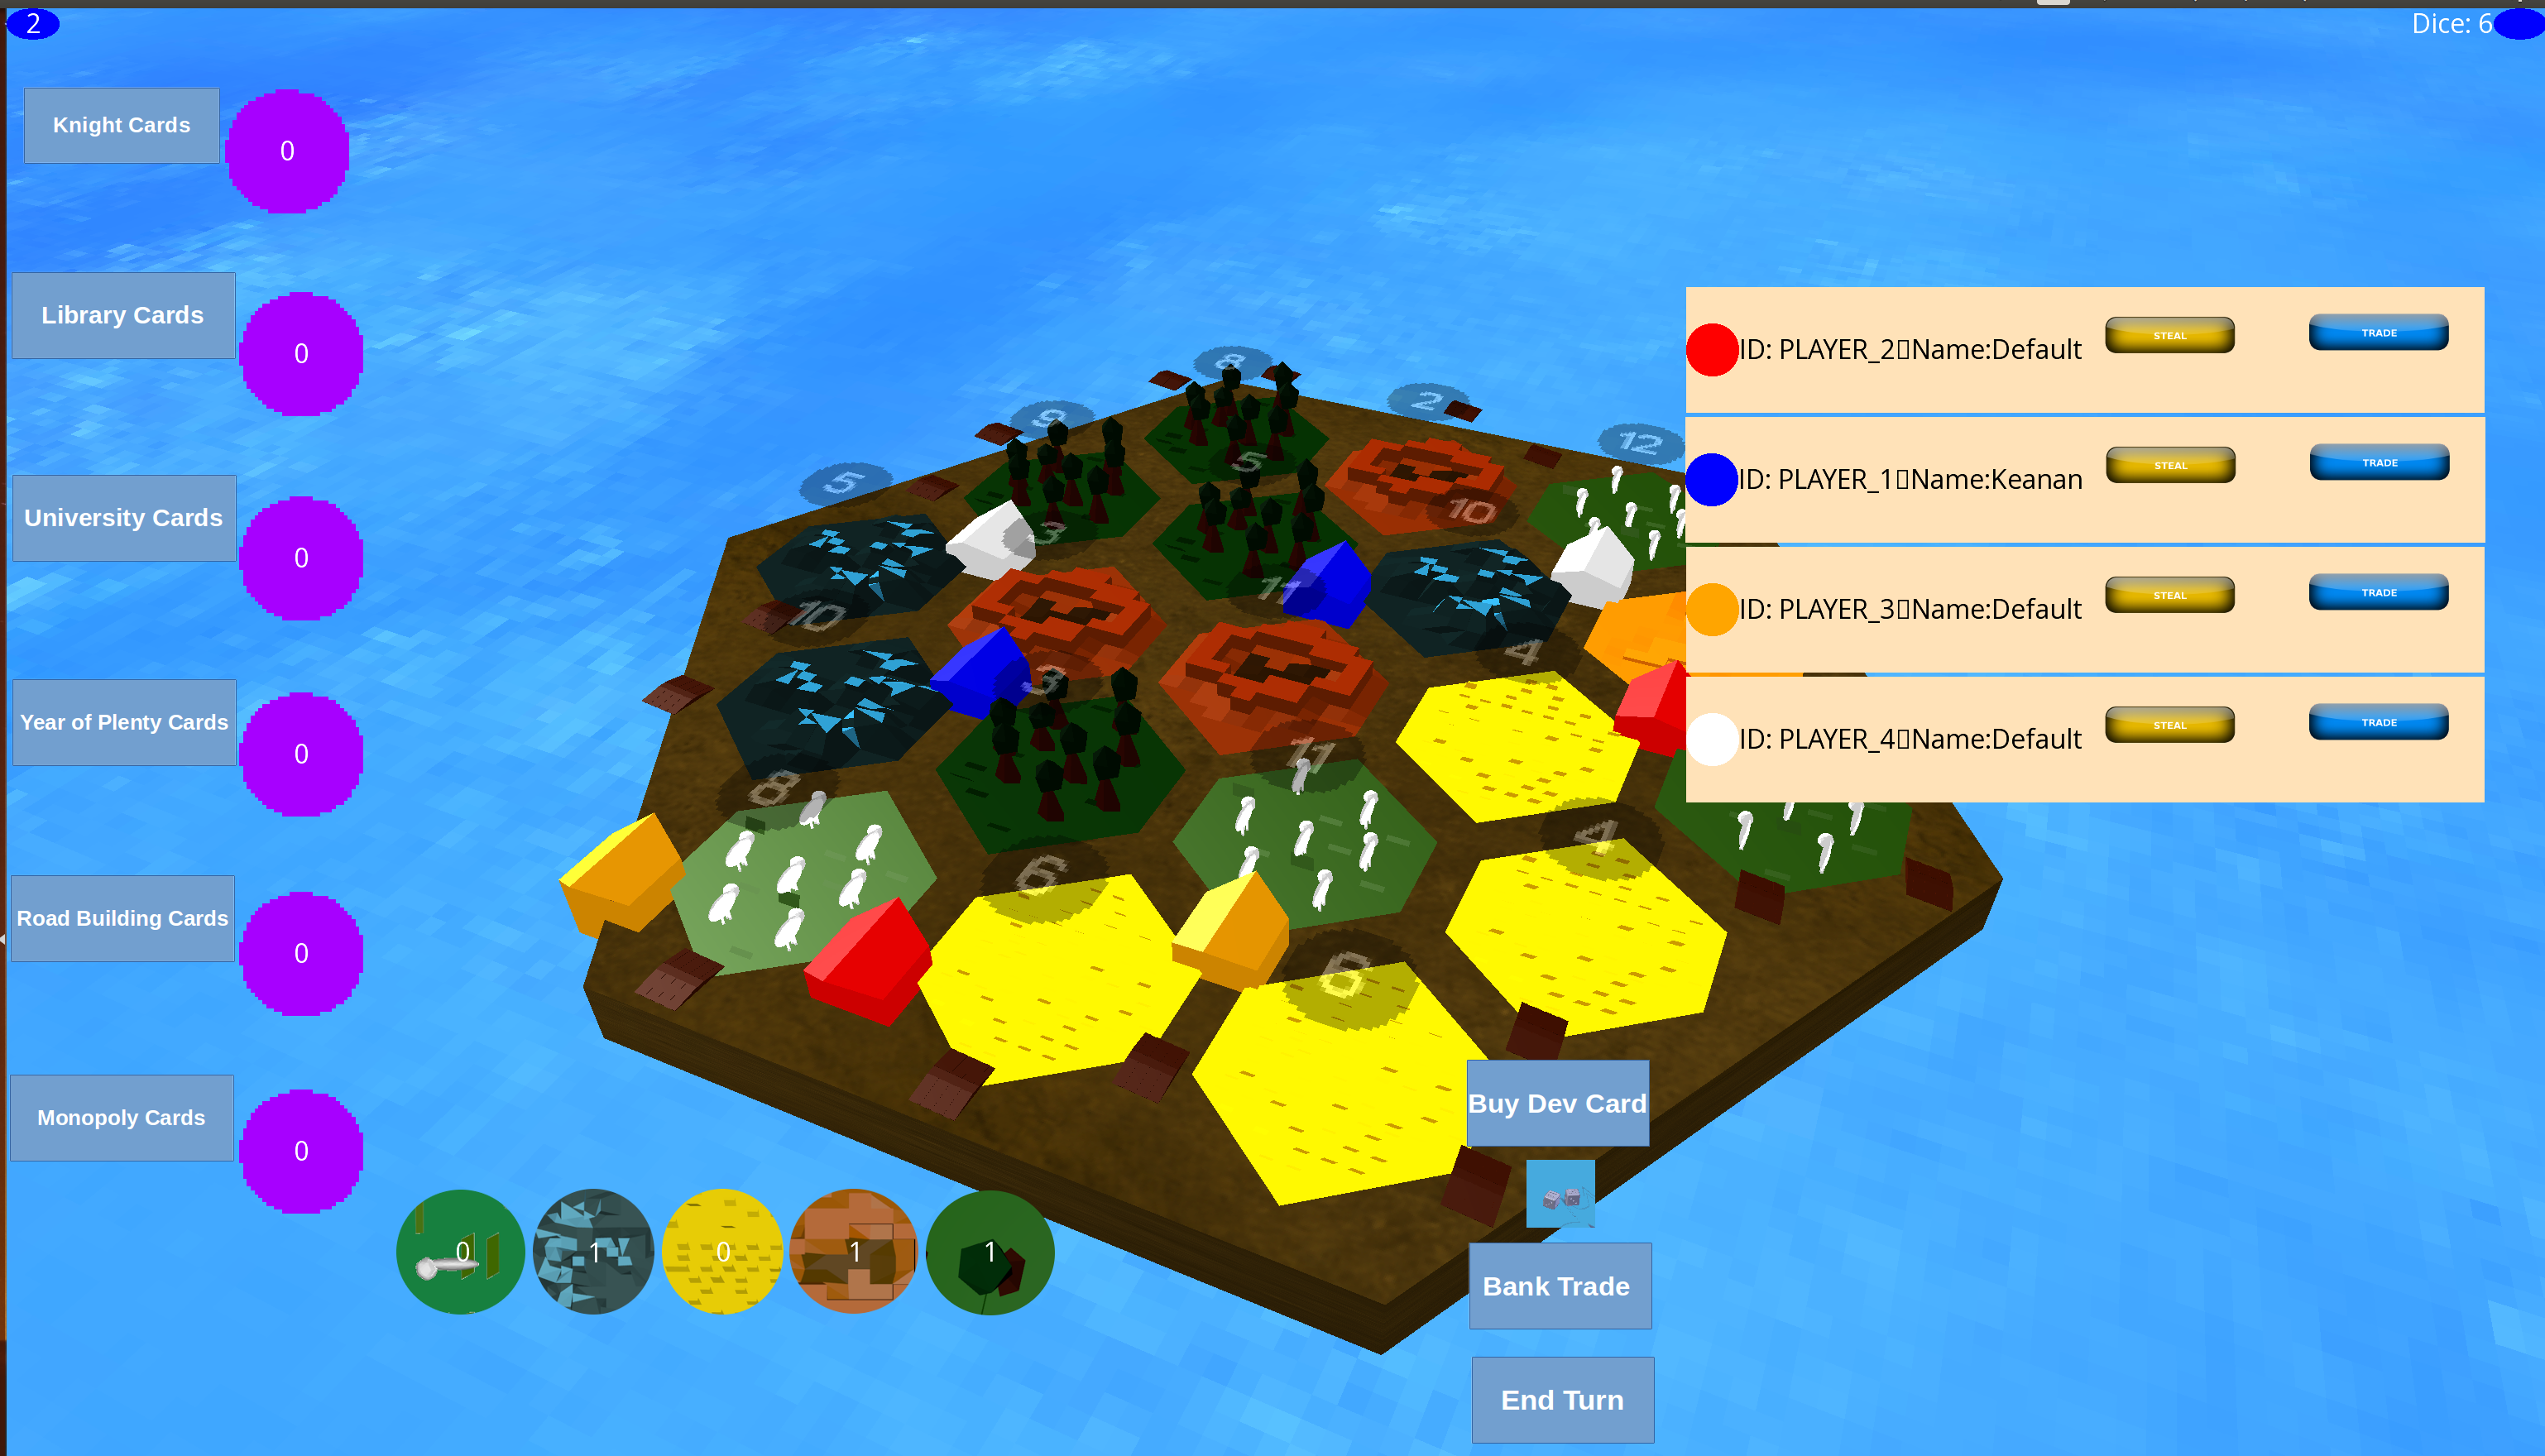
\includegraphics[width=\textwidth]{userInterface}
      \caption{User Interface for a non-AI Client}
\end{figure}
\subsection{Longest Road Implementation and Commonalities between ServerGame and ClientGame}
A few pieces of functionality that are common to ‘Game’ involve all the functions for longest road detection, the function for largest army detection, as well as the function for ascertaining a player’s new resource allotment based upon a given dice roll. The functions for longest road cover the different cases in which road lengths change based upon road location, including connection a chain, building on the end of a chain, having a new foreign settlement break a chain, or having an existing foreign settlement break a road connecting another. These functions all get invoked when a new road is built. As is in the case of a foreign settlement breaking a road, its method is invoked whenever a settlement is built instead. These methods all rely on how roads are stored in the Player class; they’re stored in lists of lists with each list representing a single autonomous chain of roads. This data structure, while involving expensive insert operations, leads to far simpler detection of longest road which happens with a lot more frequency. As such, the operation of checking longest road is far simpler in concept and complexity (just check the length of each road chain), which is a fair trade off.

Due to a player’s roads being stored as lists of lists, the methods for longest road therefore operate on these individual lists whenever a given road or settlement is built, and decide whether or not two lists need to merged, whether a settlement’s node is present in the list of edges and then also how to break up that chain into two, which chain to insert an edge into, or whether the road represents an entirely new chain. To check if an edge belongs in a given chain, all edges of each list are checked to see if one is directly connected to the new road (if they share a node). If so, then the road is added to that chain. If however the road is added to two chains, then all the elements of one list are added to the other, the former list is removed entirely, and with the new, duplicate road being eliminated in the joined chain to keep everything consistent.  For a settlement breaking a road, the edges associated with that node are checked to see if they have a road of another colour. If so, then that player’s road chains are checked for a split.

With all this logic in place, whenever a settlement or road is built, a function gets called to check for longest road. It performs any revoking and granting of the victory points (VP) associated with the longest road card. The largest army detection logic is similar in that it gets called anytime a player plays a knight development card. This function checks the size of the player’s army who currently has largest army, if any, and performs any revoking and grant of the associated victory points if necessary. Allocating a resource was the last, mentioned example of functionality common between ‘ServerGame’ and ‘ClientGame’ that is therefore present in ‘Game.’ This function takes a player colour and a dice roll, and checks all the player’s settlements to see if any is present next to a hex with a chit matching the dice roll. If so, then 1 or 2 resources are added to a map of resources to integers to be returned, depending on if the node has a settlement or city, respectively. This is repeated for all settlements, and the map can then be returned. Once all players have the resources they should be allotted for the given turn, then the maps for each player can be checked for inconsistency. For example, if during the initial process it was discovered that a given resource cannot be allotted, then this resource is eliminated from EVERY players’ map of new resources. Once this sanitisation process has completed, then the resources can be granted to each user, with the maps being converted and sent out as part of the ‘ROLLED’ event.

\subsection{Differences Between a Server and Client's view of a Player}
Similarly to ‘Game,’ ‘ServerGame,’ and ‘ClientGame,’ ‘Player,’ ‘ServerPlayer,’ and ‘ClientPlayer’ have an essentially comparable relationship dynamic in terms of how logic is allocated; as one would guess, ‘Player’ contains all logic for manipulating information about players that is common to both the server and the clients, while ‘ServerPlayer’ and ‘ClientPlayer’ contain special logic that only applies to either circumstance. For example, as ‘ServerGame’ performs a multitude of checks to see if a request lines up the given game state, ‘ServerPlayer’ entails a lot of the functionality for checking if a request lines up with the given player state. This represents a layer of functionality in the backend, as well (to be discussed further in “Server Design”). Contrastingly, ‘LocalPlayer’ doesn’t entail much logic at all, aside from a few minor things which slightly differ from ServerPlayer’s version. This abstraction allows for a lot of code re-use as well, as common functionality is shared in ‘Player.’

\section{Server Design}
\begin{figure}[hbtp]
      \includegraphics[width=\textwidth]{server}
      \caption{Server Class Diagram}
\end{figure}
The backend was designed using a modular approach, with very clear layers of functionality. The server is the top layer, which coordinates communication between all threads listening to players. It retrieves messages from each ‘ListenerThread,’ and passes these messages into a ‘LinkedBlockingQueue’ in the subsequent layer, the ‘MessageProcessor.’ The ‘MessageProcessor’ is the part of the server which reads messages one at a time, breaks them down, and parses them for accuracy and validity based upon the current game state. It keeps track of which moves have been seen and if any players have any moves which they are expected to make, and uses this information to help deduce if the received move is valid. If so, it also determines what action to take and then performs it. Often this includes going one layer deeper in the server into the ‘ServerGame,’ which acts as the authoritative state for the overall “Settlers of Catan” instance. The protocol-buffers-compatible representation of the request from ‘MessageProcessor’ is transformed into one understandable by the internal game logic, and then the action is carried out if all internal information is valid.

\subsection{Server Message Parsing}
Parsing of the protobuf class ‘Message’ is quite easy, thanks to the extra mechanisms protocol buffers entail. When a message can be ‘one of’ something, an enum is implicitly set in the protobuf object which tells you which option was set, allowing for easy retrieval. This makes parsing requests very simple, as all one needs to do is ‘switch’ on the field representing what field of the ‘Request’ is set. This tells you exactly what information to extract from the request, and in most cases then calls the appropriate method in ‘ServerGame’ to handle that request type. In the cases of chat messages or trade requests to other players, these are instead just forwarded to the remaining players. Otherwise, the internal request is sent to the ‘ServerGame’ for further processing. If the processing succeeds with no exceptions or other errors, the given request is run through a method that determines what expected moves are now expected from each individual player. These expected moves are used in determining if an incoming request is valid as well, along with other basic information like which player sent the request, whose turn it is, and similar information. Before being further parsed, the extracted request is run through a series of checks like this. Due to expected moves being so fundamental to determining if a move is valid, every request  which succeeds needs to be ran through a method to eliminate the successful move if it was already expected from that player, as well as determine if any players have new expected moves. For example, if a 7 is rolled, then any player with over 7 resources needs to send a ‘DISCARDRESOURCES’ request, and the player who rolled needs to also send a ‘MOVEROBBER’ request before the game can proceed.

\subsection{Server and Client Communication}
In thinking about the way the server should communicate with the clients, it was noted that it would have to be general enough to be able to handle a local or remote client. This would allow AI’s to be able to be run directly from the server-side as well, and for a client to be able to host a server locally. Likewise, regardless of the type of client, the Server needs to be able to be constantly listening for messages from all clients, as in some instances messages are required when it isn’t the player’s turn (I.e responding to a trade, discarding cards, etc). Due to these needs, a class ‘ListenerThread’ was created which unsurprisingly, runs in its own thread. This addresses the need of being able to constantly listen for messages, as each thread simply needs to loop listening for incoming messages from the client. When found, it adds this new message to the ‘LinkedBlockingQueue’ in the Server’s ‘MessageProcessor,’ so that the message will be handled once it’s at the front. The concurrent nature of the queue allows for each individual ‘ListenerThread’ to populate the queue without needing to worry about acquiring a lock first, given that information could be lost or corrupted if this race condition were not handled. Likewise, it means the Server’s ‘MessageProcessor’ doesn’t need to worry about this either, as it simply needs to ‘poll’ messages from the queue and process them one at a time.

To address the first need of having local or remote clients, the ‘ListenerThread’ sends and receives its messages through an ‘IClientConnection’ object, representing either a local OR remote client, as opposed to having ‘ListenerThread’ implemented strictly in terms of a TCP connection. This abstraction is necessary as it means the ListenerThread needn’t care of the underlying implementation of its ‘IClientConnection.’ The two classes which implement this interface include ‘LocalClientConnection’ and ‘RemoteClientConnection,’ and simply entail functions for sending and receiving messages from the corresponding ‘Client.’ The latter is simply a wrapper over a TCP socket, which allows the Server to be connected with remote clients, regardless of implementation (provided they adhere to the group protocol), while the former also has an object reference to a ‘LocalServerConnection’ object, which is the analogous version for a ‘LocalClient’ object (to be discussed later), thereby creating a bridge between the local client and the server (run in separate threads). This is the mechanism which allows for local AI’s to be run from the Server, or for a local Server to be run directly from a client, the combination of which would allow for an “offline mode.” In summary, ‘ListenerThread’ fulfils the aforementioned requirements, in allowing for all users to be listened to constantly (so no messages are lost or delayed), and for the sending and receiving messages regardless of the context of the connection. This means the same code can be used for having local OR networked clients, as with the correct abstraction mechanisms, the nature of the client doesn’t impact the flow of communication whatsoever -- only HOW the communication is sent.

\section{Client Design}
\begin{figure}[hbtp]
      \includegraphics[width=\textwidth]{client}
      \caption{Client Class Diagram}
\end{figure}
Given the way the ‘ListenerThread’ objects on the Server abstract over the type of connection, a Client needed to be abstracted over to indicate what components were necessary for ALL clients, regardless of implementation to be plugged into the server (either Remotely or Locally). These core components of a ‘Client,’ inherent to a ‘Client’ if they wish to hook up to our server, include an ‘EventProcessor’ (continually listens to the server, either locally or remotely, and processes incoming events while updating the state and expected moves), a ‘MoveProcessor’ (generating a list of ALL valid moves for a given turn, and if a given request is valid), a ‘TurnProcessor’ (constructing a request message and sending it off the server, either locally or remotely), and a ‘ClientGame’ (representing the overall state of the underlying game, from the Client’s perspective and to the best of its ability) all of which share a reference to the corresponding ‘Client.’ These core components are defined and are fields in an abstract ‘Client’ class, given their functionality is constant regardless of the type of client (AI vs Player, and local vs remote); this means that any actual implementation of a client simply needs to extend the abstract ‘Client’ class, instantiate its fields properly, and add any additional modules or information to maintain. This is the most modular approach possible, and means one only needs to write client logic ONCE, and can then make local and remote specialisations which override two methods (setUp and shutDown) so that it can plug into the existing code. For example, ‘AIClient’ extends Client, entails all AI logic, and is then extended by ‘LocalAIClient,’ ‘LocalAIClientOnServer,’ and ‘RemoteAIClient,’ which simply have involve different ‘IServerConnection’ and ‘IClientConnection’ objects. These different connections are of course reflected in ‘EventProcessor,’ ‘TurnProcessor,’ and ‘ListenerThread’). With those core, three relationships properly set up between client and server, no other code needs to be changed to make a local client available remotely, and vice versa.

Due to all the interacting aspects of an abstract ‘Client,’ ensuring thread-safe, consistent communication between the different components was essential. This becomes even more necessary when thinking about a client in relation to a graphical user interface (GUI), which would need to run in its own thread as well for the sake of responsiveness. For the core ‘Client,’ mechanisms needed to be introduced to ensure that as the ‘EventProcessor’ received events, that the associated ‘ClientGame’ be updated in coordination with the GUI and AI, in order to facilitate the remaining in sync of all modules with one another, and to ensure no corruption of data or other race conditions. Likewise, these mechanisms needed to be general enough so that they would function in the opposite way, as well as would accommodate future additions to the code easily. To implement these requirements, it was noted that a notion of a ‘lock’ would be needed whenever accessing or updating the ‘ClientGame,’ so that other threads would be forced to block until the resource became available. If the thread has the resource however, then it can conduct its business and subsequently release the lock, thereby allowing another thread to resume. For example, if the GUI is wishing to update the board, it first attempts to acquire the relevant lock from its ‘Client’ object, and then it can ensure that the view of the state it is getting is up-to-date and current. In order for this mechanism to be employed correctly, all participating threads that go into a client need to be spinning and waiting for the given lock at all times, if it doesn’t already have it. Due to this and for reasons discussed in the subsequent paragraph, the entire ‘Client’ class implements ‘Runnable’ (so that it may be run in its own thread). Its main ‘run()’ method is simply an infinite while loop which attempts to acquire the lock associated with the client’s ‘ClientGame’ and the one associated with the Client’s ‘Turn’ (to be discussed later), and then reads an event if available, followed by updating the state. Other threads which desire the ‘ClientGame’ then need to acquire the lock, which then essentially interrupts this thread, as it will then need to block until it can receive the lock resource once more.

\subsection{Client Event Processing}
\begin{figure}[hbtp]
      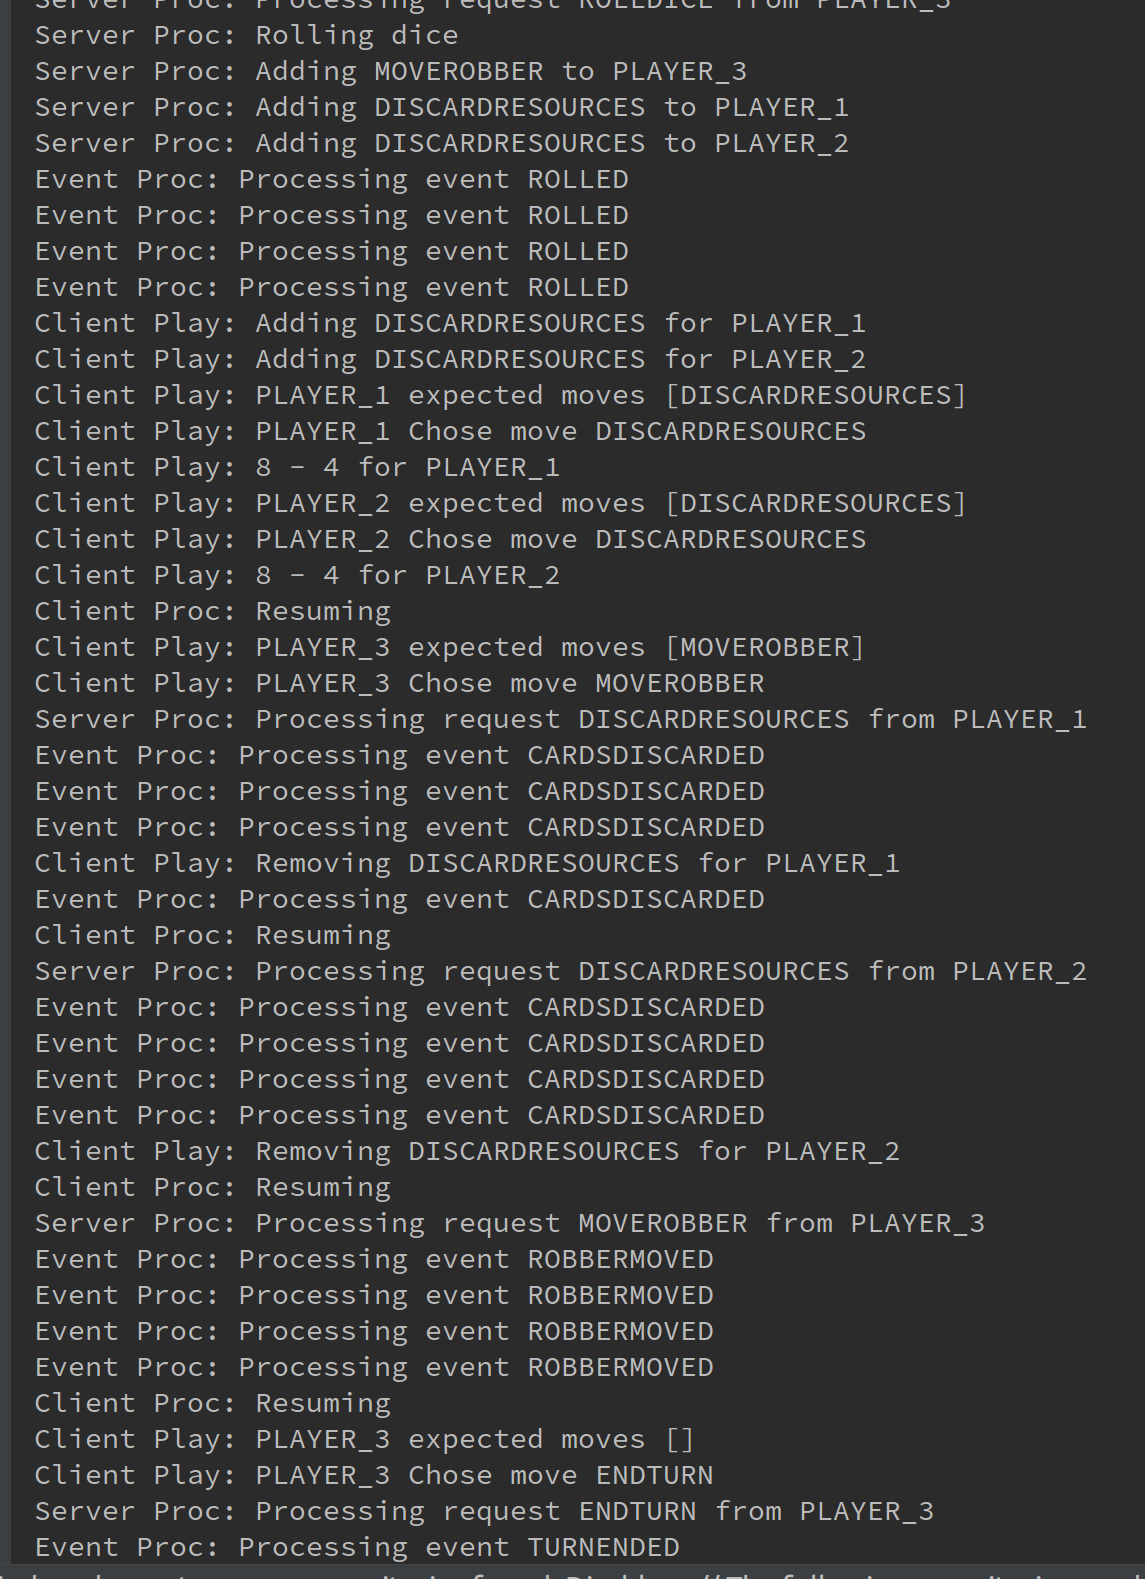
\includegraphics[width=\textwidth]{eventlog}
      \caption{Event log sample of running game}
\end{figure}
‘EventProcessor’ is intended to operate in its own thread, and has a reference to an instance of an IServerConnection. This connection, to be discussed more thoroughly later, abstracts over the nature of the connection with the server, and simply facilitates the sending and receiving of messages to and from the server, respectively. ‘EventProcessor’ only focuses on the receiving of messages; it handles the parsing of received messages and events, and then passes them off to the corresponding Client’s ‘ClientGame,’ to handle the processing of the new information about the game. The ‘EventProcessor’ needs to run its own thread as the server sends events inconsistently, unexpectedly and from all players; as such, the client needs to be constantly listening to the server so that no messages are missed. When the event processor is processing a message and stripping out the internal ‘Event’  (see “Protocol Design”), or rejecting it if it is not there, it determines the type of the event in a ‘switch’ statement, and therefore also which method in ‘ClientGame’ to call to process it further. It also runs the event through a method which analyses the event, the instigator, and any other participants to determine any new expected moves for this player (i.e. a discard request when seeing a dice roll of ‘7’ while having more than 7 resources, or a response to a trade when one is received, etc.). There are some simple checks in ‘EventProcessor,’ but it is assumed that the server has an authoritative knowledge of the state of the game meaning that these are just a formality. This is justified by the fact that if something does go wrong due to the server, the client will be unable to recover anyway. o

Before understanding how moves are sent to the server, it is important to note what a ‘Turn’ object is. The ‘TurnProcessor’ works by processing the main ‘Turn’ object in ‘Client.’ This object is quite important, as it entails all information about the current turn’s state, including dice roll, expected moves, whether-or-not it is trade phase, as well as the current information about the desired request the user wishes to make. Given the information it entails, it is no surprise that this object is also utilised and altered by the different components of a client; as such, it necessitates the use of another lock as well. The ‘Turn’ object is the primary way for a generic ‘Client’ to set up moves, regardless of how it provides moves to the ‘TurnProcessor’ (AI, Player, etc.). Essentially, the ‘Turn’ object entails a field for ‘ChosenMove’ which is an instance of the enum type used in a ‘Request’ (see Protocol Details), as well as fields which describe further information about all possible request types, with relevant pieces of information filled in. For example, a ‘Turn’ object representing a ‘BUILDSETTLEMENT’ move would have the ‘chosenMove’ field set to ‘BUILDSETTLEMENT,’ as well as having the ‘chosenNode’ field filled in as well. This object extends to all requests in a similar way, meaning it therefore is capable of encapsulating all possible information about a desired move. This object type is therefore used in multiple scenarios, such as generating moves (MoveProcessor.java), as well as in forming potential moves and updating the main ‘Turn’ object so a move can be processed and sent.

\subsection{Client Sending Moves}
‘TurnProcessor’ operates with the same ‘IServerConnection’ that the Client’s ‘EventProcessor’ has, but conversely only focuses on the sending of moves to the server. In having all communication with the server abstracted over with one object, the ‘IServerConnection’ is the only element on the client-side that is needed to separate a remote connection from a local one. A ‘RemoteServerConnection’ is essentially just a wrapper over a java TCP socket, while a ‘LocalServerConnection’ simply just has a reference to the Server’s corresponding ListenerThread’s ‘LocalClientConnection.’ This ‘bridge’ is facilitated through two ‘LinkedBlockingQueues,’ one of which is in ‘LocalServerConnection’ and the other of which is in ‘LocalClientConnection.’ These queues represent a stream of messages being received from the other end of the connection, and in this way, messages can easily be passed between a generic, local client and server (AI, Player, etc). ‘TurnProcessor’ as a class focuses on forming the request to be sent to the server, and then it calls a method to validate the request from the client’s associated ‘MoveProcessor.’ It forms a request by, provided it has the lock, looking at the Client’s ‘Turn’ object, ‘switching’ on the ‘chosenMove’ field, and then extracting out the relevant information. These two bits are used to form a ‘Request’ object (see  “Protocol Design”), which is then sent to the associated ‘MoveProcessor’ to be validated against game state and expected moves. If the request is valid, it can then be sent to the server via the Client’s ‘IServerConnection.’

\subsection{Client Move Validation and Generation}
The ‘MoveProcessor’ class is tasked with validating moves based upon the current game state. The game state it has is the ‘ClientGame’ object that the associated ‘Client’ instance has. This class has a method for each unique type of request that dictates if a given move would be valid, based upon the current game state. These methods entail checks such as if it’s the player’s turn, if they can afford the thing they are about to buy / build, if the move is expected, and similar logic specific to each request. For checking a given request based off of known expected moves, the list of expected moves is first checked to be empty. As briefly mentioned before, the expected moves are retrieved and updated via the cross-thread ‘Turn’ object, associated with the given ‘Client.’ If the expected moves are empty, then remaining checks for the given move can be carried out. If however, the list of expected moves is NOT empty, then if the given request type is NOT present in the list of expected moves, the move is invalid. If the request is in the list, then additional checks for the request may be carried out. Here, expected moves are NOT eliminated from the list as this is done with the client’s ‘EventProcessor;’ since events verify whether a move was indeed carried out, then this is the only place where expected moves can be added or removed based on principle. This is necessary due to the fact that some moves require multiple elements to be fulfilled. For example, playing a monopoly development card involves first sending a move to play a monopoly development card. If this succeeds, then the player must then send a ‘choose resource’ request. Likewise, playing a ‘Year of Plenty’ development card involves two subsequent ‘choose resource’ requests, and moving a robber entails moving the robber, then submitting a player to steal from. If the client were to not maintain when moves are expected, AI’s would need to have hard-coded elements to remember when they had to play a certain move after another. Having the expected moves integrated into a client’s fundamental move and event processing modules makes move validation for any client infinitely more seamless.

‘MoveProcessor’ also entails functionality for generating all valid move possibilities, as this is used in some way for all sensible, generic implementations of a ‘Client.’ For example, an AI could use this functionality so it doesn’t have to generate moves itself, and likewise a GUI could use it to display valid options and give visual cues to the user. This functionality works by systematically checking every move possibility, and running the corresponding method in ‘MoveProcessor’ for checking the  validity of that request type. Using these functions as a filter, all move possibilities can easily be filtered. For example, an internal function in ‘MoveProcessor’ called ‘genBuildingPossiblities’ returns a list of all BoardElements (‘Node’ objects, ‘Edge’ objects, and ‘Hex objects’) which can be built upon. This method looks at all nodes and edges in the Client’s ‘HexGrid’ (stored in ‘ClientGame’), retrieves the local player for this ‘Client,’ and checks if the ‘Player’ can build on the given node or edge, or upgrade the given settlement. This is performed through the corresponding functions in ‘MoveProcessor,’ which are implemented in terms of analogous functions in the abstract ‘Player’ class. These are common to both a ‘ServerPlayer’ and ‘LocalPlayer;’ that is, it simply checks if the given player can build there. If so, a ‘Turn’ object is constructed using the ‘BoardElement,’ and added to a list. With all building possibilities sorted, then each remaining function in ‘MoveProcessor’ is called with each possible valid input. If the function returns ‘true,’ indicating that the move option is valid, then ‘Turn’ objects are constructed with the given request type and additional info. This forms a master list of valid moves, and is subsequently returned.

\section{User Interface Design and Architecture}

\section{AI}
\subsection{AI Architecture}
\begin{figure}[hbtp]
      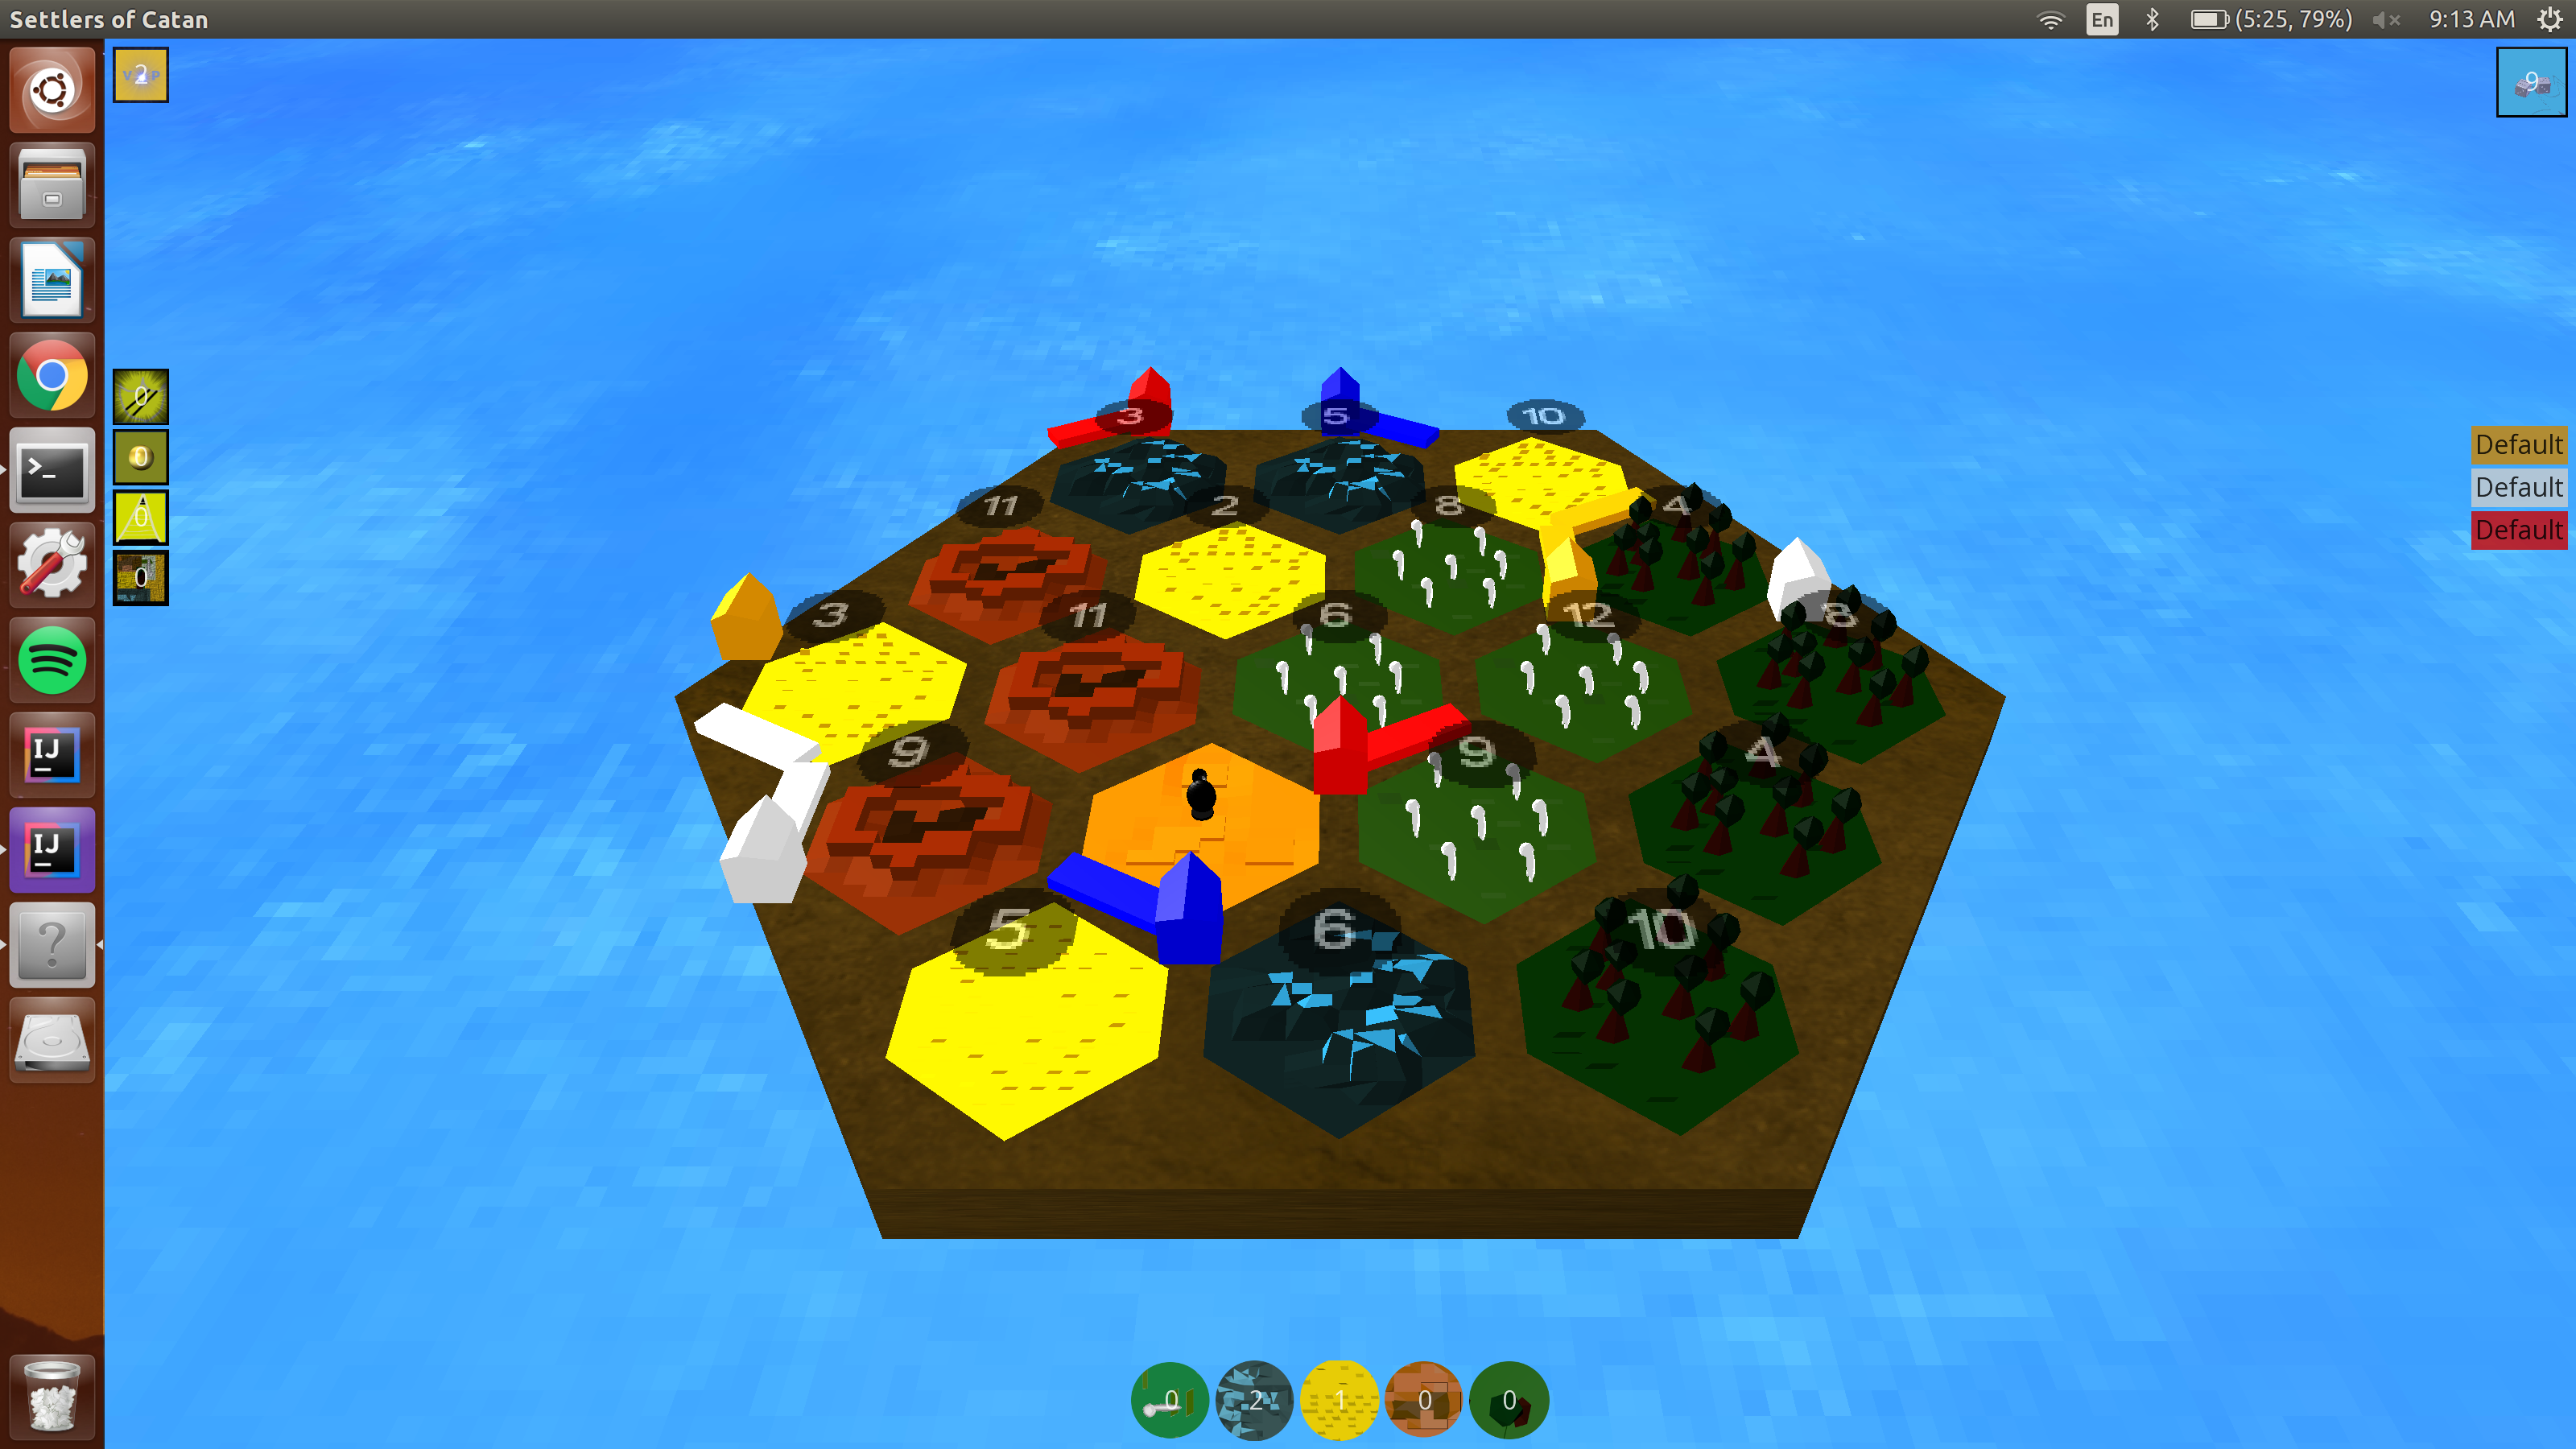
\includegraphics[width=\textwidth]{userInterfaceAI}
      \caption{User Interface for an AI Client (Buttons disabled)}
\end{figure}
To begin with coding the AI, the generalisation of what is means to be a client needed to first be fulfilled. With this, then the AI could be implemented through little additional code, beyond the AI logic, of course. This is due to the way in which AIs are able to hook into the Client framework. Essentially all an ‘AIClient’ needs to do is to extend ‘Client,’ override Client’s run() loop, and implement some AI which has a method of retrieving all valid move possibilities.  With this, then each one simply needs to be ranked in some way, with the one with the highest rank chosen and sent via the client’s ‘TurnProcessor.’ Luckily, ‘MoveProcessor’ is an aspect of every ‘Client’ implementation, and thus any AI simply needs to do for getting move possibilities is to call on ‘MoveProcessor,’ as it already knows how to retrieve the list of valid moves for the given state of the turn. This, in turn, means that an AI doesn’t need to know or care about which moves are expected; in the case of a move being expected, the returned list from ‘MoveProcessor’ would merely only contain moves of that type, provided there are no other constraints present. This means an AI simply needs to go through the stream of valid move possibilities and assign a rank, vastly simplifying its job and reducing the amount of code redundancy. If the AI had this functionality from ‘MoveProcessor’ directly, then it would essentially be causing the processing and recording of this duplicate information. The current approach is vastly more efficient and modular.

In order to keep the ‘AIClient’ as simple as possible, it was made abstract similarly to ‘Client,’ as well as given an abstract object as a field, ‘AICore,’ which entails all processing and decision-making functionality. The only thing this leaves for ‘AIClient’ is to have its own run() method; its version of run() differs from that of the one in ‘Client,’ as this one needs to incorporate logic for making moves as well as processing events. The loop structure remains entirely identical, however, in that the loop tries to acquire locks before performing a given action. The run() method for ‘AIClient’ is an infinite while loop (for all intents as purposes), which acquires locks, tries to process an event, releases locks, sleeps, acquires locks, calls an abstract method for generating a move from the ‘AICore’ if given conditions are met (it is the AIs turn OR a move is expected from the AI (i.e. discard request)), and then releases its locks again. Alternatively an ‘AIClient’ could’ve used the same run() method as ‘Client,’ if the ‘AICore’ implementation ran in its own thread as well, however this presented an issue in terms of synchronisation; for example, this meant that an AI couldn’t move onto another move until it received some sort of feedback in the form of an event. This was attempted, and simply involved the ‘AIClient’ hanging and having a lot more downtime. In this case, the AIClient’s behaviour with locks, making moves and processing events essentially amounted to synchronous behaviour anyway. Likewise, it was a lot more complex of a program, with one extra thread for each ‘AIClient,’ and harder to debug and ensure thread safety. The current manifestation of AIClient’s run() method produces no noticeable downsides, and is worth the trade off. Likewise, it is all that needs done to ensure that the AI can hook up with the server.

\begin{figure}[hbtp]
      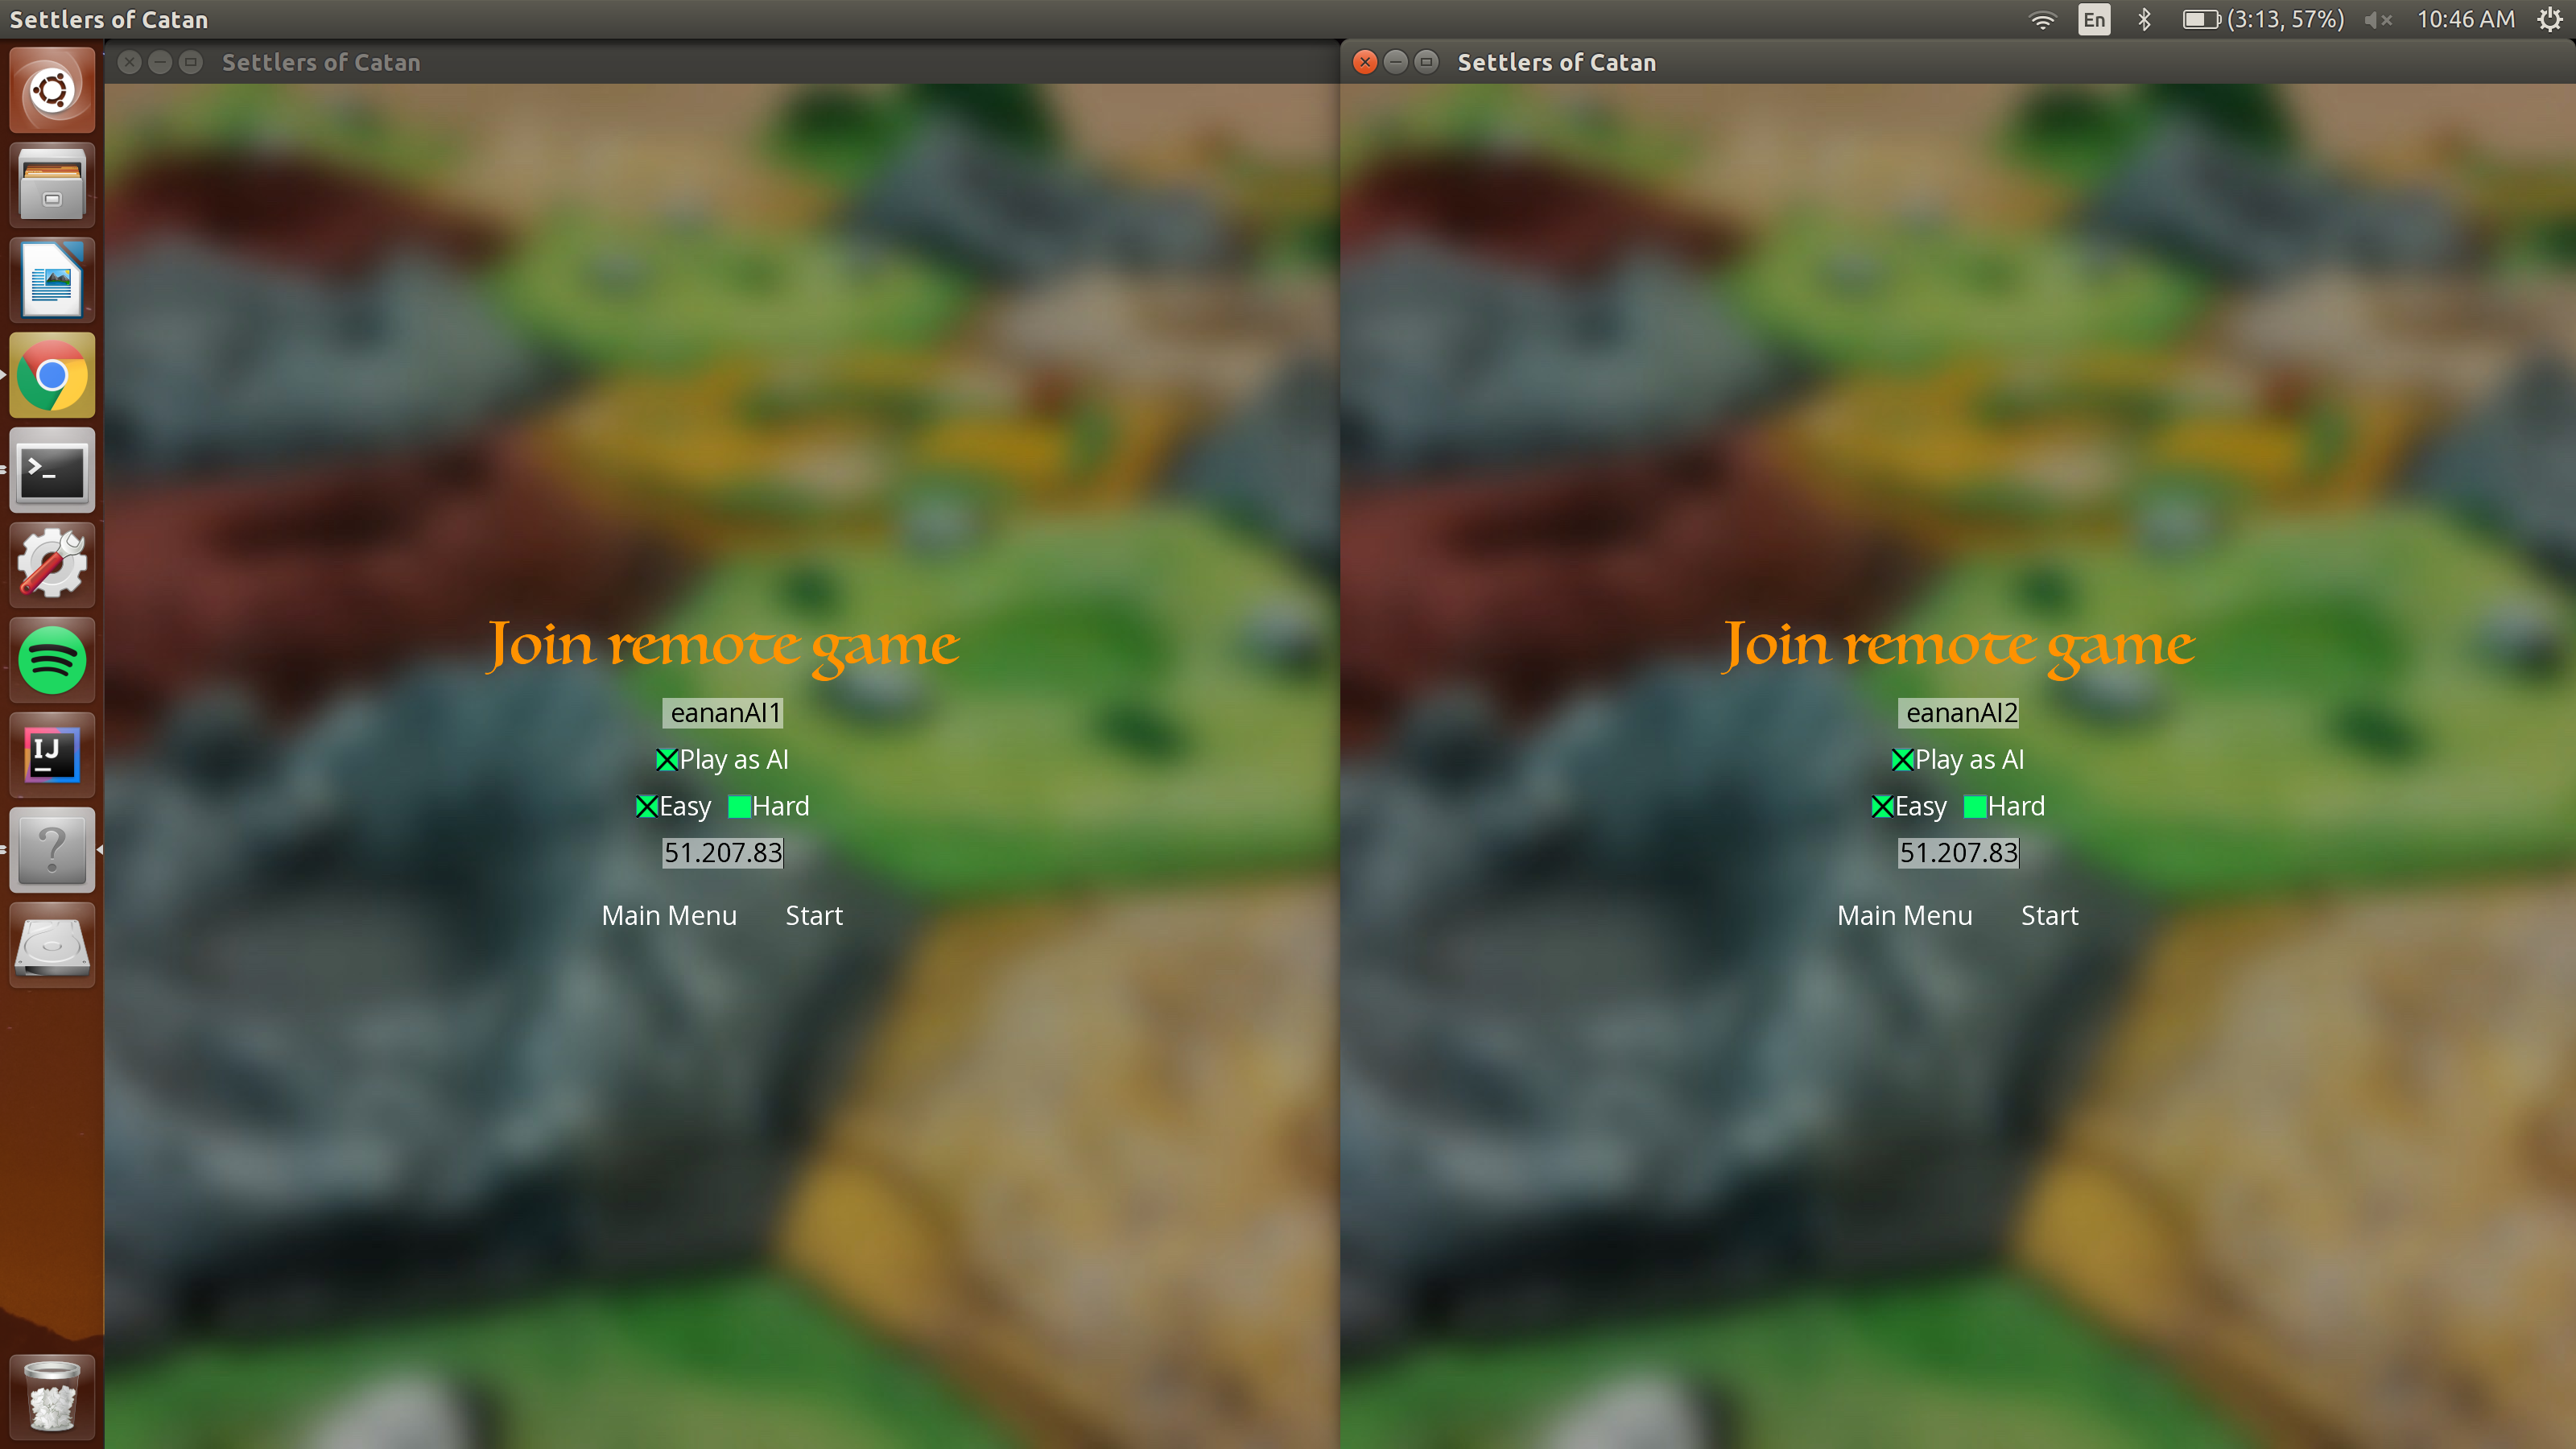
\includegraphics[width=\textwidth]{aiSetUp}
      \caption{User Interface for choosing AI difficulties for two players.}
\end{figure}
\paragraph{Abstracting over the AI logic unit, allowing for different difficulties}
In order to actually implement the AI’s logic, an interface ‘IAI’ was written to describe the methods needed by an AI in order to properly hook up with an ‘AIClient.’ The main one is the performMove() method which coordinates the relationship between all the remaining abstract functions defined in the interface. These include getMoves(), rankMoves(), selectMove() and selectAndPrepareMove(), while the remaining functions defined in ‘IAI’ are to be implemented in the actual implementations of ‘AICore.’ This approach was decided upon as it involves the most amount of code re-use as possible; this is because any AI logic implementation will need a method of retrieving valid moves, ranking them, selecting them, and preparing the move for being sent off to the AIClient’s associated ‘TurnProcessor.’ Ranking moves is the bit in which the actual AI logic comes into play, and could involve anything from simply assigning numbers, to a full-blown Monte Carlo Tree Search or a something similar. As of now, AICore’s implementation of rankMoves() simply switches on the ‘chosenMove’ field of the given ‘Turn’  (from the overall list of possibilities), and then calls the appropriate abstract heuristic function. AICore’s current implementation of selectMove() simply takes a list of all optimal moves (that is, all ‘Turn’ objects which share the highest ranking), and randomly chooses one. With the current structure, all one needs to do to write an AI that can interact with a server is to create a class which extends from ‘AICore,’ and simply implement the given functions for heuristic calculation. ‘AICore,’ as described above, already handles the manner in which these components interact. In the described manner of architecting AIs, implementing a random AI simply entails overriding every heuristic function to return the same number (i.e. 0). In this way, every possible move will be a part of the ‘optimalMoves’ list parameter to AICore.selectMove() (that was generated from rankMoves()), and the function will simply choose a random one.

Given that ‘AIClient’ can have any implementation of ‘AICore’ as its underlying AI logic processing unit, the described system for AI implementation is flexible, easily extensible to future heuristics, and conducive to iteration and improvement. Likewise, this also means that ‘AIClient’ and its children classes are the only classes needed to hook up ANY implementation of ‘AICore’ to the server for playing a game. ‘AIClient’ has three classes which inherit from it: ‘RemoteAIClient,’ ‘LocalAIClient,’ and ‘LocalAIClientOnServer.’ The latter entails an ‘AIClient’ which operates directly from the server, operating on a different thread, while the former two represent an ‘AIClient’ running with a GUI, remotely and locally from the server, respectively. The former two are analogous to ‘RemoteClient’ and ‘LocalClient,’ respectively, and essentially entail the exact code as the corresponding class (except for which class it inherits from, and a few other things).


\subsection{AI logic}
\subsubsection{Design}
Ideally we would have wanted to have at least three levels of AI player:
Easy: An AI that would play random moves
Medium: An AI that chooses its moved based purely on heuristics
Hard: And AI that uses A* or Monte Carlo search algorithms to choose moves
Due to time constraints however we only managed to implement the first two difficulty levels. As the Easy difficulty makes moves randomly, all further discussion about the AI will be in relation to the Medium difficulty level AI.

\paragraph{Strategy}
After a carefully observed game of Settlers of Catan with the team, we realised what strategies exist and what strategies are superior to others. For example one person’s aim was to win the game by upgrading to cities quickly. One error in this strategy is that the person did not think to expand through roads and settlement and hence were left with options of buying development cards and trading resources. Their buildings( settlements/cities) were located around hexes that had essential resources, but most of the hexes were very unlikely to return anything as the dice rolls on these were unlikely to occur( i.e 10-12). They therefore chose to trade before making any moves in order to maximise the likelihood of being able to build any item in a certain round, making them a very impulsive and impatient player. As assumed, this person had the least victory points at the end of the game. 

On the other hand, another person placed their initial settlements wisely and chose to go with the “largest road” strategy (this was made easy due to a stable resource flow), which granted them two additional victory points while being ahead of the other players for the majority of the game.

The third person and winner of the game used a mix of strategies, but the main aspect that helped him win was that he bought development cards throughout the game and only played them as the end of the game when it would put him above the winning threshold of victory points and ahead of the second strategic player.

What we deduced from this:
It is important that you build roads so you can build more settlements 
This will stabilise your resource flow 
More likely if settlements are placed around hexes with likely dice rolls
You could gain 2 additional victory points
Cities are only worth considering if you have a solid foundation of settlements
Development Cards are most useful at the end of the game when you are close to winning

Hence the main strategy of the AI is to prioritise aspects of the game in the following order:

\begin{description}
\item[$\bullet$ Roads] - prioritised throughout the game while aiding building of settlements
\item[$\bullet$ Settlements] - prioritised at the beginning of the game while advancing
\item[$\bullet$ Cities] - considered once advanced to a stable game state 
\item[$\bullet$ Development Cards] - considered and prioritised at the end of the game or when an opponent is close in terms of victory points.
\end{description}

The AI will expand quickly by building a lot of settlements and roads quickly. This will give our AI access to better settlement locations early on (stabilising resource flow )and will increase its chances of getting the longest road. 



\paragraph{Resources}
The first thing we considered was which resources we wanted our AI player to prioritize. As our main strategy is to have the AI expand quickly and build as many settlements and roads as possible. To this end, we decided to make ore our lowest priority as it is the only resource that is not used in building settlements or roads.
While deciding how to prioritize the remaining four resources we looked at how often our AI would require those resources. We observed that bricks and lumber are required for both settlements and roads it made a lot of sense to make those our top priorities as it would allow the AI to better achieve its goal of expanding quickly. Our third priority is grain as it is a necessary resource for more items than any of the others which provides a strong case for it being the most useful resource. However, two of the three items that can be bought for grain also require ore and as we had decided to make ore our lowest priority it would not have been sensible to prioritize grain any higher. After these discussions we agreed on the following resource priority order:

\begin{description}
\item[$\bullet$ Bricks]
\item[$\bullet$ Lumber]
\item[$\bullet$ Grain]
\item[$\bullet$ Wool]
\item[$\bullet$ Ore]
\end{description}

Resources Implementation:
The prioritization of these resources is implemented using an ArrayList containing each resource type that ensures that the AI attempts to acquire each resource and does not attempt to only acquire the most favourable one. The ArrayList in the Rank Node class is modified at each call of the rank method by ranking the resource in ascending order, making the most scarce resource always a priority. Hence, because we take care of prioritization in the initial road and settlement placements of the game, we can now focus on establishing a balance between getting the right amount of resources and getting the right resources.

\paragraph{Settlements}
Settlement Placements and City Upgrades:
	At the beginning of the game, potential settlement placements are ranked on two criteria. The first of which is how many of the four prioritized resources they give the AI access to. The second criterion is the probability of receiving any of the resources as indicated by the dice roll required to gain those resources so locations adjacent to resources that require dice rolls of  between five and nine (excluding seven) gain priority. The first part of the ranking is mainly dependant on the number of unique resources a potential settlement would provide to the AI such that the AI does not prioritize a location that meets the second. criterion well but only provides a single resource type over a location that does not provide the best probabilities of receiving resources but provides a greater variety of resources.

Settlement Placement and City upgrades Implementation:

During the game the AI decides to prioritise the settlements that are around the nodes that have resources that are scarce rather than the initial prioritization of resources.This is realised through the resource queue that is updated each time a road or settlement placement is evaluated. Nevertheless, the AI prioritises settlements near hexes with a more likely dice roll. This is necessary to ensure that a continuous stream of resources is at the hand of the AI so that the main aim of expansion can be realised. 



\paragraph{Road Placements}
\begin{figure}[hbtp]
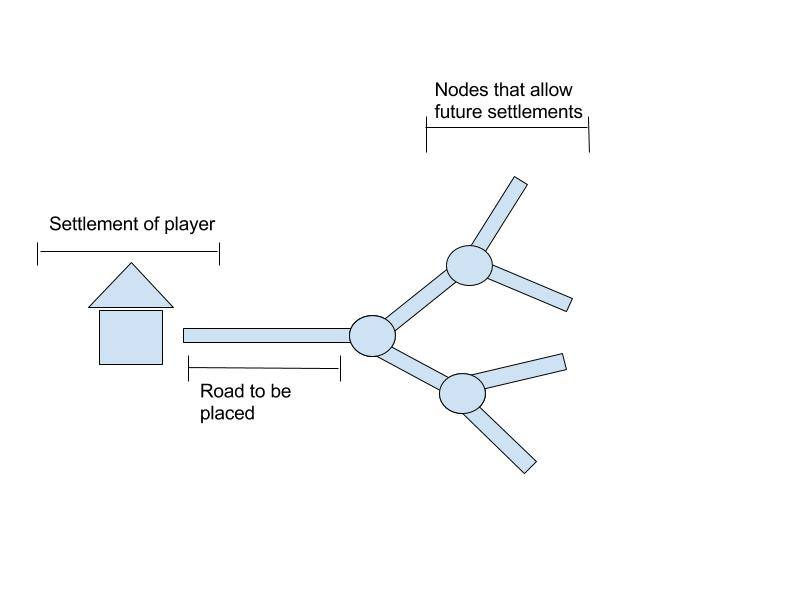
\includegraphics[width=\textwidth]{AIRoadPlacement}
\caption{How road placement is determined}
\end{figure}
For each potential new road location there are two different situations that can apply to the location. The particular situation must be identified before the edge can be ranked properly.    
 The first situation is that the road would be connected to a node that a settlement can be built on. In this situation we decided that the most important factor would be the feasibility of the connected node as a settlement location. As such, the road is ranked based on the rank that the node would receive if it were being considered as a settlement location.
The second situation is that the road is not connected to a node on which a settlement can be built such as an edge connected to a settlement. When ranking an edge under these conditions we first take into account what the edge is connected to. If the edge is connected to an opposing settlement then the dge gets ranked down as this would stifle expansion. If the case is that the edge is connected to one of the AI player’s settlements then the edge gets ranked up slightly as a road built on that edge would contribute to the longest road goal without harming the AI’s ability to expand.  If the edge is connected to an empty node then we rank the edge based on the road building options that it would open up to the AI player. Edges in this situation are ranked based on the number of valid settlement building options they could potentially provide.

Road Placements Implementation:
	This mechanism is implemented in rank New Road in the easy AI class. The road in the first situation is ranked higher than the second situation as it helps our aim of expanding as quickly as possible. If the road to be placed is connected to a settlement, making it impossible to place a settlement at the other end of the road, we first evaluate the edges going away from the node of the road to be placed that is not connected to the settlement

Then it looks at all edges connected to that node that are not the edge on which the road is to be placed. The rank increases every time it discovers that the nodes that allow for future settlements are not occupied by opponents’ settlements.If one of these nodes is occupied by an opponent it decreases the rank of the road, if it is the player’s own settlement the ranking increases as it allows you to expand quicker.

\paragraph{Trading}
The trading has been implemented to accept requests that offer resources that the AI is lacking or in need of. If it does offer such resources, the ranking for the trade is increased. In turn, if the trade requests resources that the AI has plenty of, the ranking is increased as it would not hurt the AI to lose these resources.


\paragraph{Discarding and Stealing Resources}
Discarding Resources:

For situations in which it is necessary to discard resources we attempt to work our way up our resource priority list. For this we consider bricks and lumber as having the same priority and the same consideration is given to grain and wool. As we are discarding resources based on priority, the AI will first discard any ore it has before looking at grain and wool and finally, if no other options are available, the AI will discard bricks and lumber. For the resources that are grouped, the AI will discard whichever resource it has the most of before discarding the second.

\paragraph{Moving the robber}
When choosing which player to target when given the opportunity via rolling a seven or playing a knight card the AI will attempt to target the player with the largest number of resources and the most victory points. While there were a few ways we could do this such as trying to calculate which players have which resources we felt like it would make sense for our medium AI to make a simpler choice and target the most valuable player. The most valuable player in this case is defined as the player with the greatest number of victory points and resources.


\subsubsection{Development Cards}

\paragraph{Playing Development Cards}
Development cards are ranked lower than roads and settlements due to our strategy

\begin{description}
\item[$\bullet$ Knight Card] As The Knight Card lets you move the robber, it gets a basic ranking as moving the rubber allows the AI to get resources that help it advance quicker. Apart from that there is no other benefit of playing this card (not considering the Victory points that are automatically assigned to a player).
\item[$\bullet$ Road Building Card] When evaluating this card we find the player with the longest road to get the length of the longest road and then compare it to our own road to see if 2 additional roads will give us the longest road award. Additionally, this card still helps us to expand quickly, hence it is ranked higher than the rank card.
\item[$\bullet$ Year of Plenty Card] As this card allows you to get 2 resource cards it checks if the AI is in need of 2 or less resources to build a road or a settlement. If the AI has enough resources for these 2 tasks, it evaluates if we are in need of one resource card to upgrade to a city. 1 has been chosen as we do not want to waste a development card on upgrading to a city and expansion is our strategy.
\item[$\bullet$ Monopoly Card] When the AI is given the opportunity to play the monopoly card, it checks to see if it has a settlement or city by a port which would enable it to trade the cards that it would gain at a better rate than with the resource bank. If so it ranks higher, but if it has no access to a port it gains the standard ranking of 1.
\end{description}

Due to the group protocol, it is no longer possible to keep the remaining development cards from the other players until you play them. The victory points earned from them and some of the development cards mentioned above are added immediately to the player’s total victory points.

\paragraph{Buying Development Cards}
	This has been given low priority due to the points we derived from our game which are explained above. The AI therefore tries to keep the number of development cards throughout the game at a minimum. The default ranking is decreased if the AI can afford to build or upgrade to cities. At the end it is also decreased by the number of development cards the AI already has, making it very unlikely to buy development cards when other moves are available.


\section{Intergroup protocol and the process of integration}
\begin{figure}[hbtp]
      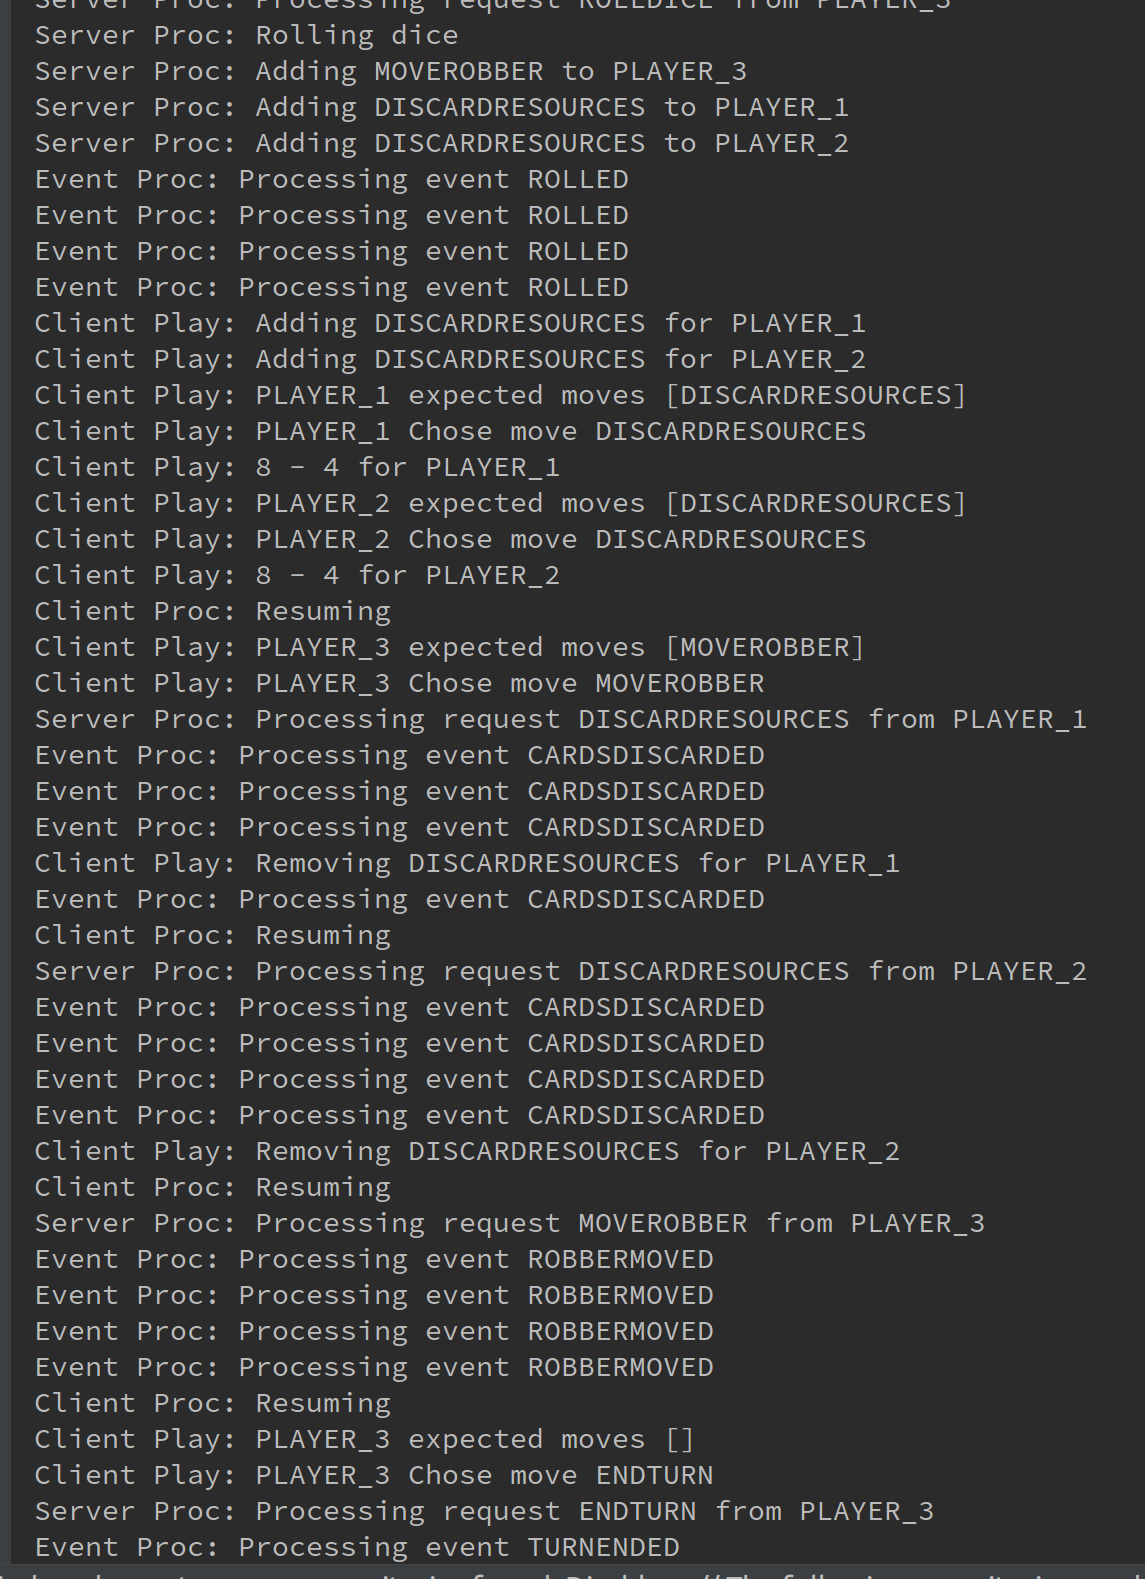
\includegraphics[width=\textwidth]{eventlog}
      \caption{Event log sample of a running game}
\end{figure}
The intergroup protocol design became pivotal to how this implementation was written, organised and structured. A group representative, Keanan, attended nearly every intergroup meeting (aside from once or twice when external obligations came into play) and worked heavily to write the protocol and provide alternative approaches and perspectives (advancing this group’s stakes in the matters at hand). For example, in order to begin coding over Christmas holiday, this group member wrote a protocol using Protocol Buffers for our group to work off of. This was based on knowledge of what the group protocol would need to entail, but at this juncture, the intergroup protocol was too minimal to provide anything to go off of. This led to the foundation of our code base, backend, and server, and the original plan was to map our internal protocol to whichever one the groups eventually decided upon. This proved to not work as well as planned, as far messier code was written than had been intended. Likewise, it involved an entirely new module to do the actual translation. Due to this, our group representative began being more active in group meetings, and worked to bridge the gaps in protocol definition that still needed to be worked out. Overall, the protocol that was written for our group entailed a more rigid, verbose protocol that was more transaction-based; that is, if one wanted to play a monopoly card or steal from a player, it was all done through one message. This was decided on as it was decidedly simpler than the alternative, in which state and expected moves had to then be maintained.

Contrastingly, the exact opposite approach was taken in the group protocol; requests have been broken up into their logical constituents, and are sent independently from one another as it, admittedly, better replicates the flow of a board game. For example, in “Settlers of Catan” when playing a year of plenty card, one would tend to play the card, and then subsequently decide on which resources they wished to receive, as opposed to doing it all at once. This methodology has been extended to every request type, and thus necessitated the maintenance of state and which moves are expected on both the client implementations and the Server. Due to the fundamental contrast in group approach and internal approach, the decision was made to simply migrate the existing code base entirely to the group protocol (once it became finalised enough). This in turn, involves a much more unified and intuitive code base, as much less translation between messages types is necessary.

\section{Collaboration and Team Process}
\begin{figure}[hbtp]
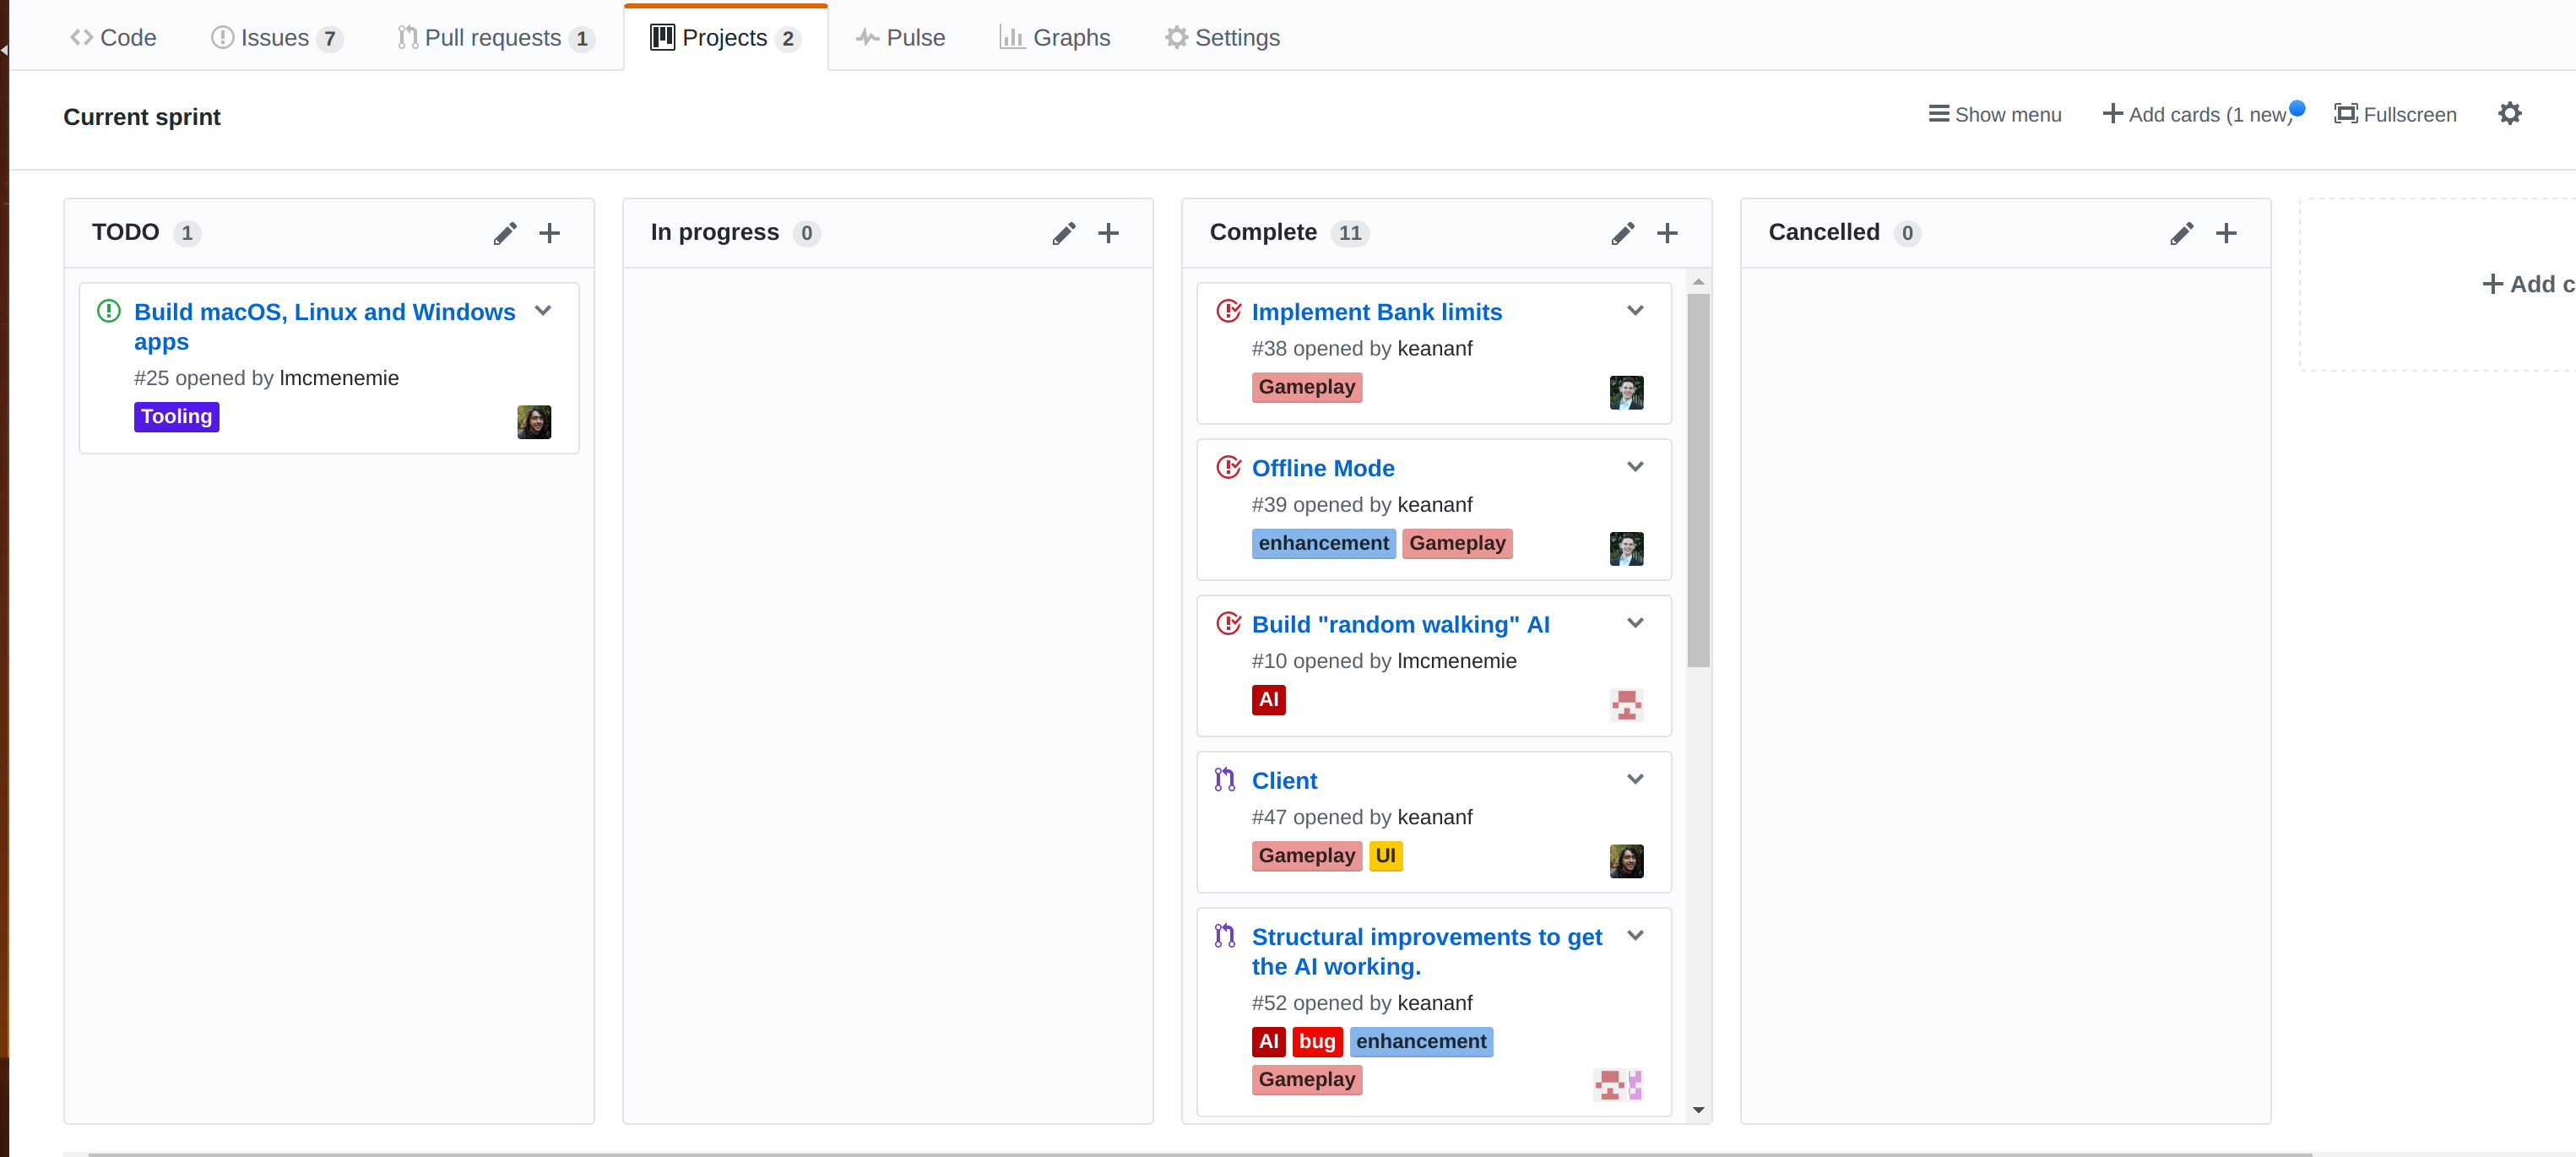
\includegraphics[width=\textwidth]{githubProjects}
\caption{Sprint that was nearly finished and documented using GitHub projects}
\end{figure}
The team functioned by essentially splitting into a front-end, ai, and back-end team, where the former consisted of Liam and Bethany, the middle of Jack and Christa and the latter of Keanan. These choices were made predominantly due to interest and skill in the aforementioned areas. The team utilised github for all version control, and had it integrated with Travis CI (Continuous Integration) to aid in the build process. As such, the 'master' branch was protected to disallow any commits directly into it; instead, major changes needed to be submitted via pull request, the build then needed to clear, and then a code review needed to take place before the merge could be official. This process was used for large changes to the code base, but proved impractical for smaller changes and iterations, primarily due to other university obligations and timing constraints. The group also used GitHub's Projects feature and issues to keep track of what work needed to be done, who needed to do it and when it was supposed to be completed by. Each task in the scrum board could be assigned, described, attached to a particular project or sprint, and given a certain topic so the task's priority level could be thoroughly kept track of. Prior to utilising GitHub's project management features, the group tried using Trello for similar online management of the project. It proved to be more cumbersome than it was worth, and the group switched to Github's project management features due to its close integration with the rest of our code base.

Keanan also served as the group representative for the intergroup protocol meetings, and contributed to the GitLab repository which housed the protocol buffer files (.proto). This meetings took place weekly or bi-weekly, and involved extensive communication about the merits of certain design decisions. 

\section{Evaluation and critical appraisal}
\textbf{Evaluating the work with respect to the original objectives. The section should also critically evaluate the work with respect to related work done by others. It should compare and contrast the project with similar work in the public domain, for example as written about in published papers, or as distributed in software available to the team.}

\subsection{Catan Universe}
Catan universe is a free, online, multi-platform version of Settlers of Catan, and almost exactly mirrors the game in terms of feel, appearance, and interaction. This is probably considered the most well-realised adaptation of the popular board game.

\paragraph{Comparison}
One of the primary advantages this implementation of the game has over ours is the clicking-and-dragging method in which most of the moves are played; this lends itself to replicate the feel of the board-game, as it appears as though you are directly moving the pieces onto the board, and playing / revealing cards to other players. Another advantage, which our implementation shares thanks to Java and libGDX's cross-platform capabilities, is the ability to play this game across varying devices and platforms. Their version also extends nicely to mobile platforms as well, whereas we haven't had time to properly test this. Its animations provide nice feedback for the user as well. Our implementation shares the addition of a game log and a chat board, however these are more limited than Catan Universe's. Given that we were able to make an implementation of Settlers of Catan that enjoys similar features to a professional version, albeit more limited / worse versions, this is a good implementation to base our successes and weaknesses on.




\section{Conclusions}
\textbf{Summarising the project, emphasising key achievements and significant drawbacks, and discussing possible future directions for the work.}
\paragraph{Group Protocol and our Group's achievements.}
In conclusion, this group was able to achieve all of what we set out to achieve, despite issues with team-work, equal allocation of features, and coordination with other groups. AIs can work locally or over the network, a server can be connected to locally (through threading) or over the network, and all of Settler's of Catan's game logic was accurately represented and produced. The group protocol's last revision took place a little over a week before the final submission deadline, which meant making multiple groups' implementations work together almost an impossibility. With that said, our group's representative was heavily involved in the inter-group coordination, and thus we were able to network with Group I with little-to-no issues first time around. This was also made additionally difficult in having the client be a fat client; this meant there was a considerable amount of time and effort that went into maintaining the synchonousity between our own client and server, let alone having them work with others. Our group is quite happy with the end results. In hindsight, coordinating an intergroup protocol between this many groups proved to be an incredibly large undertaking, one which was severely underestimated by most groups involved. We were one of the only groups to successfully play multiple full games with another group's implementation. 

\paragraph{Teamwork}
In the end, despite all the issues with teamwork, our team proved to work better together the closer we got to the deadline. Several group members pulled all-nighters and did everything they had to do to meet their obligations to the group. While some of the more ambitious goals were not able to be completed, such as the implementation of expansion packs or a larger board, we feel that with more time, it would be very interesting to see what we could accomplish.   

\paragraph{Acknowledgements}
We are particularly grateful to our supervisor Edwin Brady, who provided considerable support to all of our team members, helped make the meetings fun yet also constructive, and always pointed us in the right direction. He helped keep us on track to meet our goals, applying a healthy amount of pressure when necessary, and was a pleasure to work with overall. 

\section{Testing summary}
\textbf{Describing the steps taken to debug, test, verify or otherwise confirm the correctness of the various modules and their combination.}
To test this project, an entire unit test suite was implemented which tests the core backend, functionality and game logic, as well as if the server and client are successfully able to parse a message from the intergroup protocol and deal with it accordingly. There are countless tests in the backend which ensure that the correct exceptions get thrown when they ought to (for edge cases), as well as that “normal” use cases are covered as well. This ensures that all the game logic works as it should on the server side, and that the client is able to update its game state accordingly.

Aside from pure functionality testing, countless testing was done with AIs, clients and servers, to ensure that everything could communicate appropriately given all circumstances, expected and unexpected. AIs were tested using the main method in LocalServer.java, which simply starts up an off-line server with four AIs running directly off of it. This was used to ensure that AIs could successfully play through the initial phase with no issues. This also allowed tweaks and polish to be done to the move processing units of both the client and server, as the way in which expected moves were set up needed to be perfect to avoid errors or “hanging” AIs; this occurred if the server expected a certain move while the AI in question didn’t realise. Largely, the root cause of this involved the Client and Server going out of sync in terms of which resources the given client had; this meant that the server could expect a 'DISCARDRESOURCES' move while the Client thought it was perfectly within the resource cap of 7. This meant the server would prevent the entire game from proceeding until this given move was received, which it obviously never would be. This implementation features an additional protocol message that sends the user their resources as the server has recorded. This was used for debugging these inconsitencies between the server and the client, given the client's 'fat' architecture, as well as is used by the AIs if they ever become out of sync with the server. This happens VERY infrequently, making this particular issue incredibly hard to debug and solve. As such, this message was kept in the final implementation so as to prevent the AIs from hanging indefinitely. With all these bugs sorted and tested thoroughly for validity and reproducibility, it could be said with certainty that the application as a whole has been throughly tested.

Another area of testing involved ensuring the implementation of the Server and all the manifestations of a Client to work with other groups. This included playing a game against another group's server via RemoteClient, hooking up a RemoteAIClient to another group's server, as well as having other groups' AIs and normal clients hook up to our own server. In al cases, games were able to be completed due to the common group protocol across all groups' implementations.


\begin{appendices}

\subsection{Project objectives, specification and initial plan}
As submitted during the year.
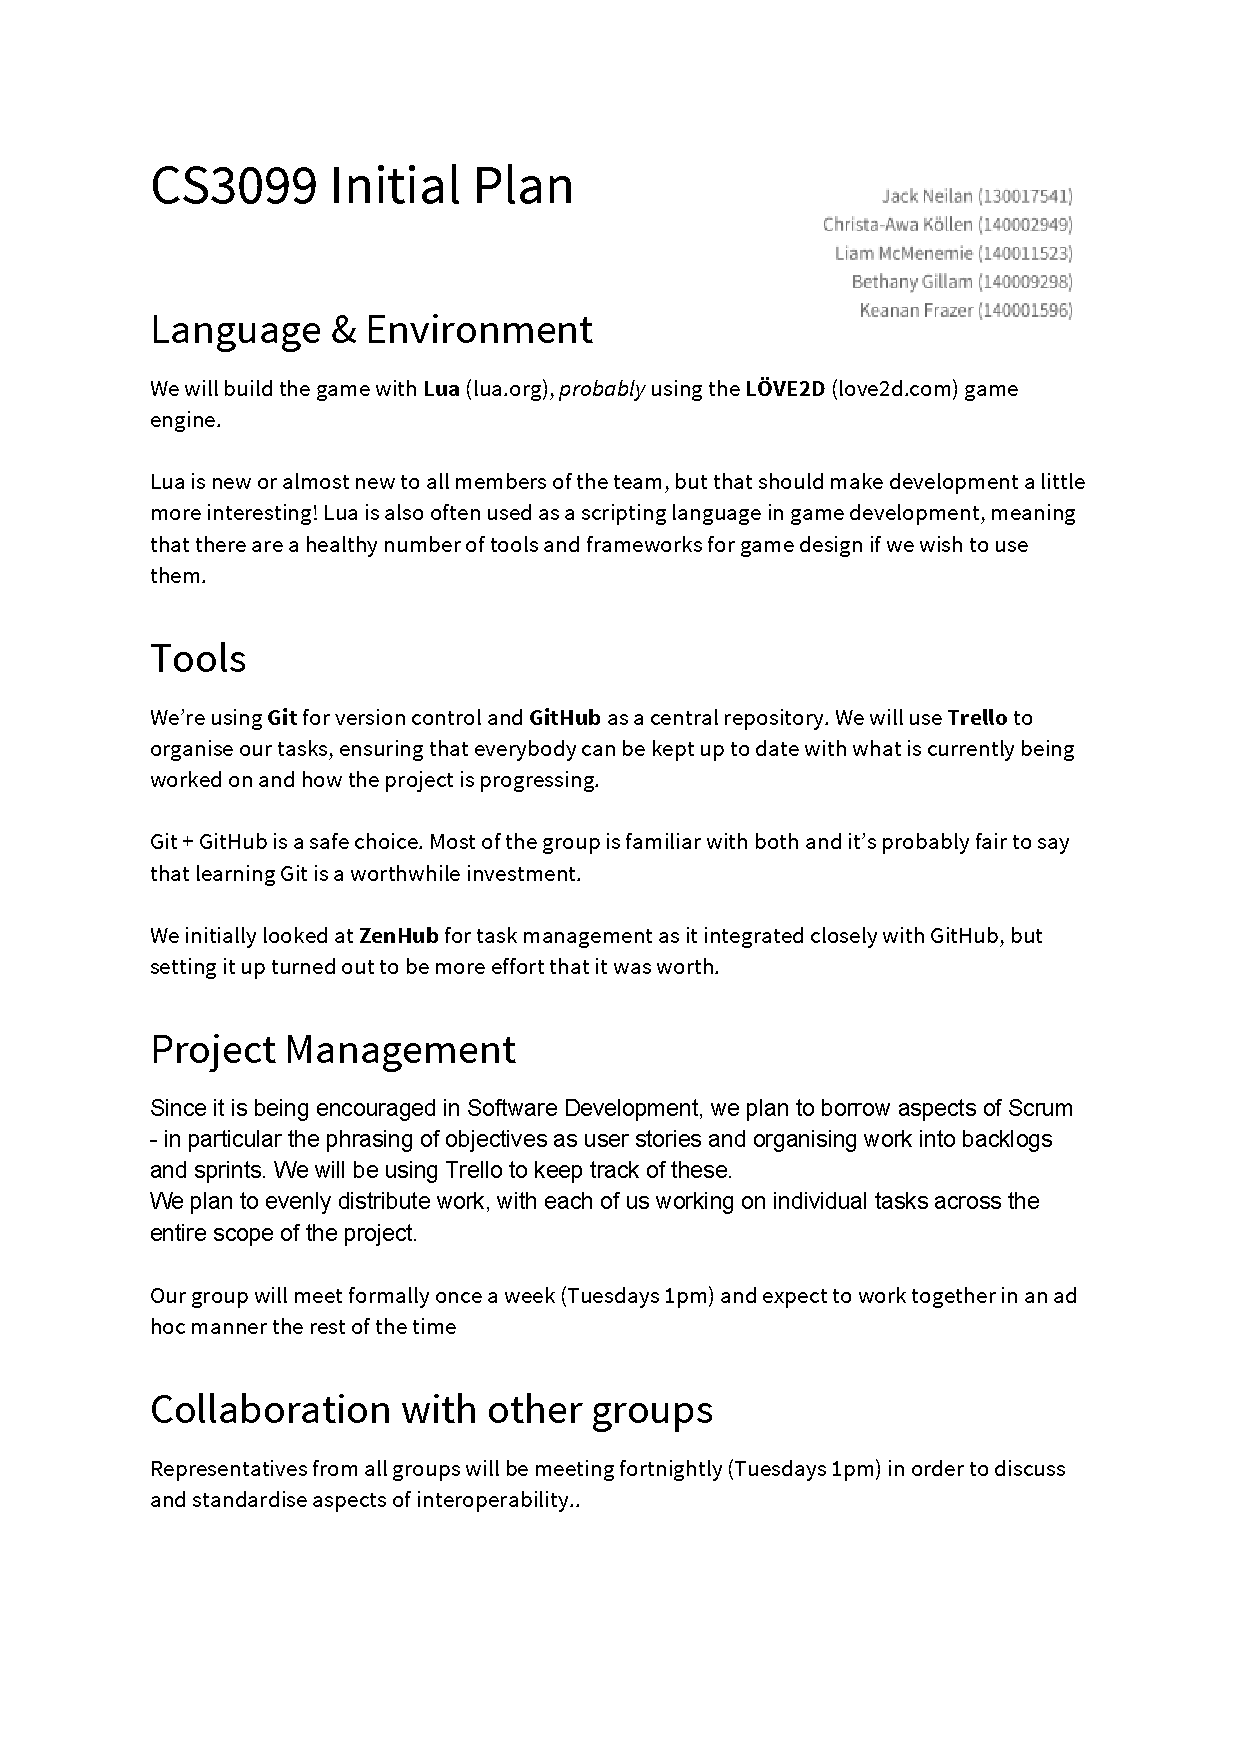
\includepdf[page=-]{InitialPlan.pdf}
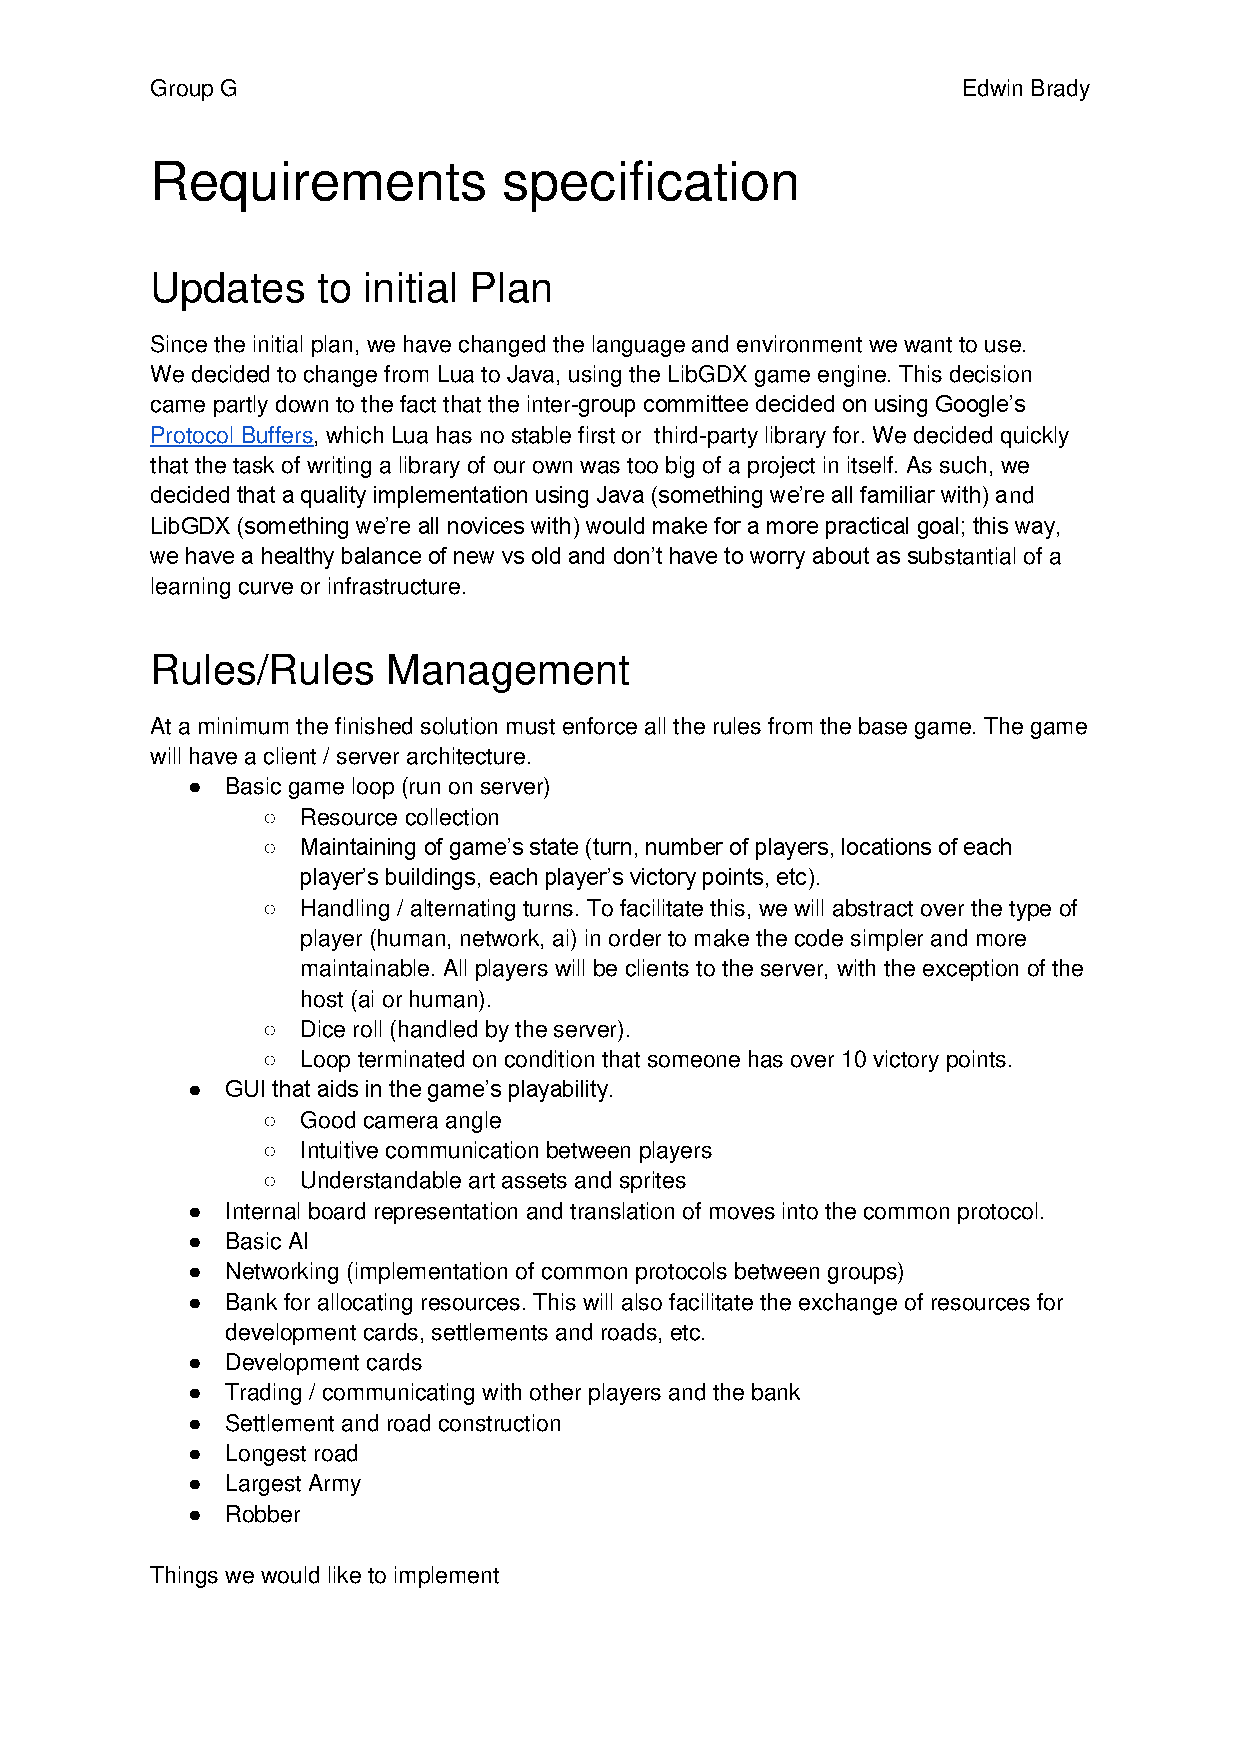
\includepdf[page=-]{RequirementsSpecification.pdf}




\subsection{S2 Interim report}
As submitted during the year.
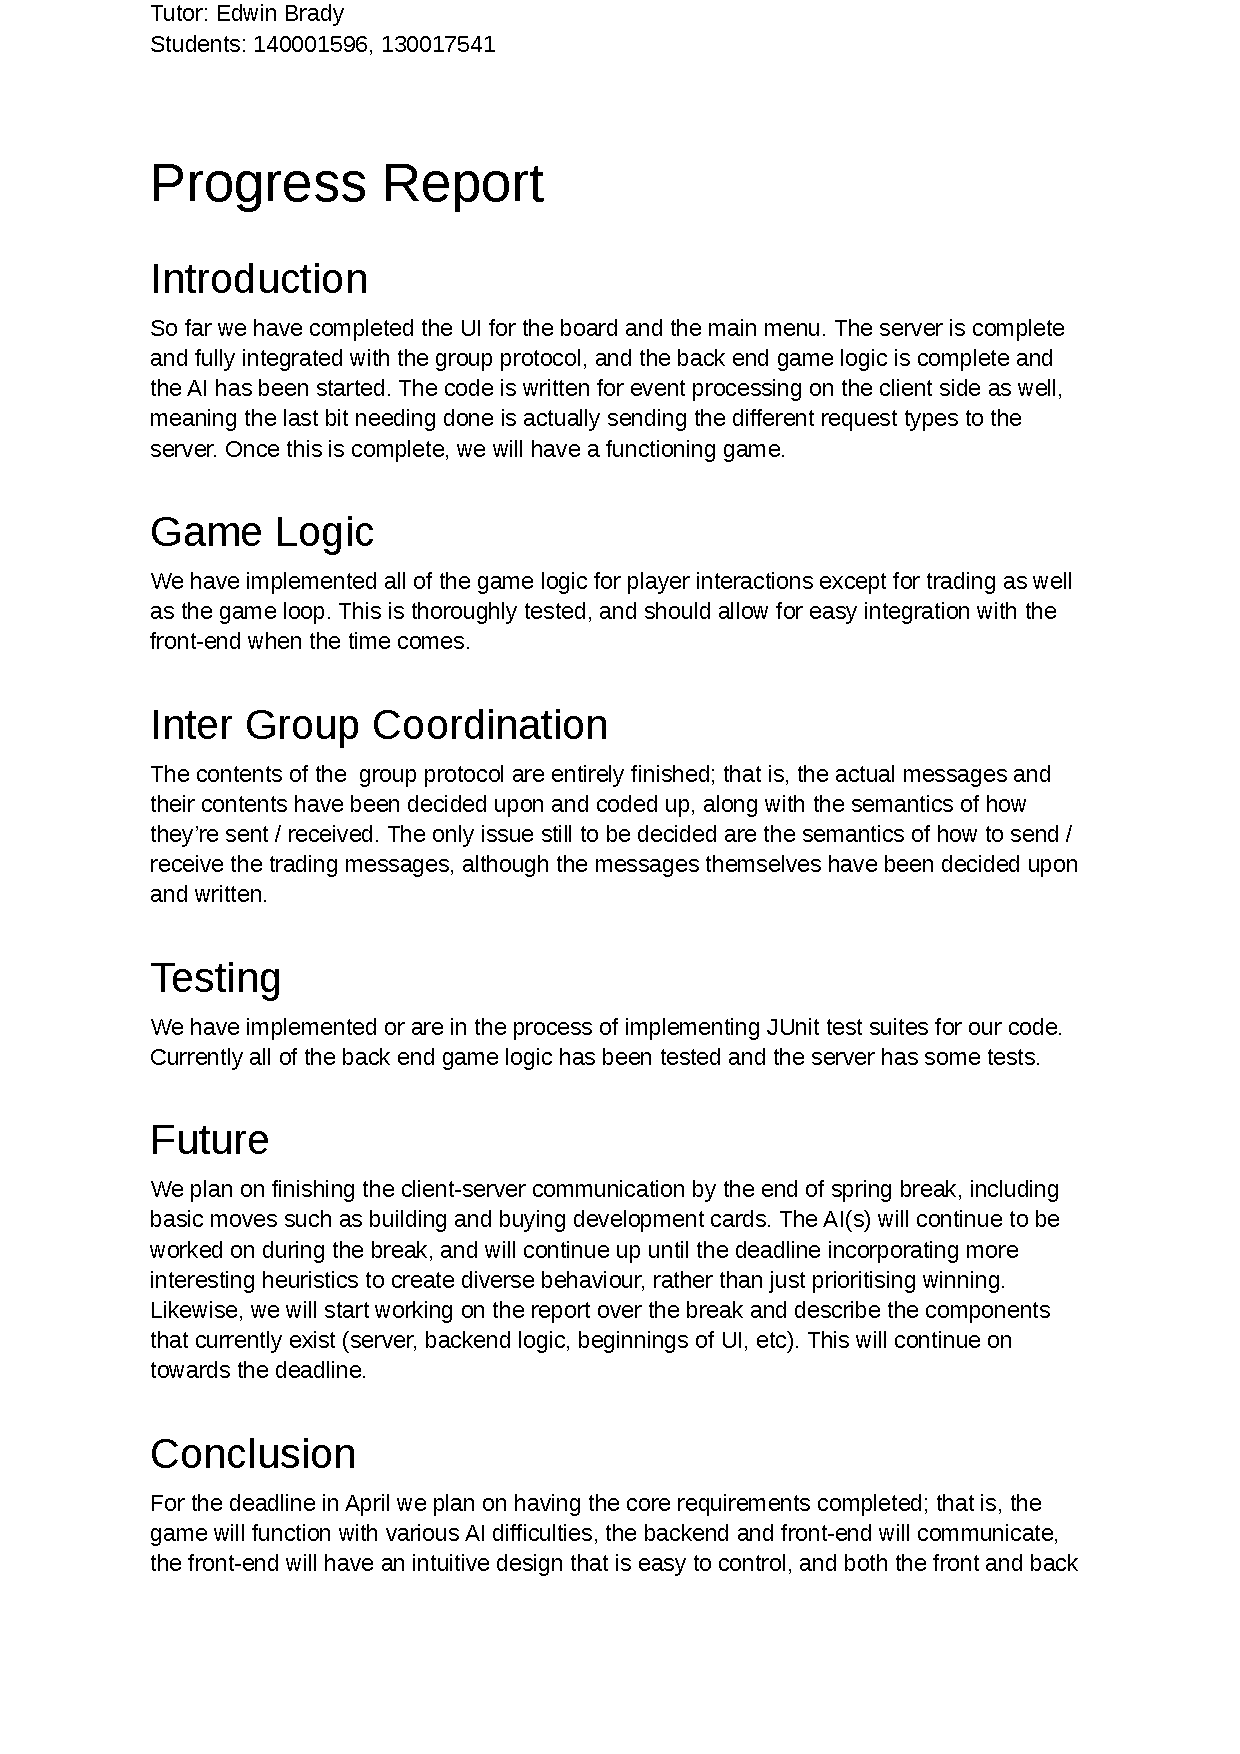
\includepdf[page=-]{ProgressReport.pdf}


\end{appendices}

\subsection{User manual}
\textbf{Instructions on installing, executing and using the system where appropriate.}




\printbibliography

\end{document}
